\documentclass[11pt]{report} %size of font and type of layout
\usepackage[a4paper,margin=1in]{geometry}

\usepackage{pgfplots}
\usepackage{tikz}
\usepackage{xfrac}
\usepackage[super]{nth} %allow 1st, 2nd by typing \nth{1}, \nth{2}
\usepackage[title,titletoc,page]{appendix} %for using appendices
\usepackage{graphicx} %have images
\usepackage{chngcntr} %be able to make figures go 1, 2, 3 instead of 1.1, 1.2, 1.3, etc
\usepackage{subcaption} %have subfigures
\usepackage{wrapfig} %be able to wrap text around figures
\usepackage{amsmath} %a way to typeset maths
\usepackage{amssymb} %able to type maths symbols
\usepackage{textcomp} %so we can use \textdegree to get degree symbol
\usepackage[parfill]{parskip} %remove paragraph indentation
\usepackage{setspace} %be able to set line spacing
\usepackage{tocloft} %more control over table of contents, list of figures, etc
\usepackage{ltxtable} %get tabularx split over pages
\usepackage[english]{babel} %english-specific charaters and language rules
\usepackage{url} %type urls
\usepackage{parskip} %space between paragraphs
\usepackage[UKenglish]{isodate} %change date format
%\usepackage[hang,flushmargin]{footmisc} %no indents in footers
%\usepackage{verbatimbox} %able to use addvbuffer to change spaces before and after tables
\usepackage{pdfpages} %insert PDF pages
%\usepackage{titletoc} %create a small table of contents at the start of each section
\usepackage{microtype} %improves spacing between words and letters
\usepackage[nodayofweek]{datetime} %use \today to get the date
\usepackage[inline]{enumitem} %have inline lists
\usepackage{fancyhdr}		%for getting customized headers
\usepackage{lastpage}		%enable getting the total of the pages
%\usepackage{floatrow} %use for indicating figures' sources
%\usepackage{showframe} %show margins on page
\usepackage[hidelinks]{hyperref} %hyperlinks in pdf
\usepackage{cleveref} %automatic referencing
\usepackage{bookmark}
\DeclareGraphicsExtensions{.pdf,.png,.jpg,.eps} %can just give images' names
\usepackage{epstopdf} %allows for encapsulated postscript vector images, better quality and scalable
\usepackage[none]{hyphenat}		%kills all word breaks that were in annoying places

%--------------------------heading spacings----------------------------%
\usepackage{titlesec} %be able to change title settings
	\titleformat{\chapter}{\normalfont\huge\bfseries}{\thechapter.}{1em}{} %have number before chapter title
	\titlespacing{\chapter}{0pc}{0pc}{0pc} %have nice spacing after chapter title {indent} {before} {after}
	\titlespacing{\section}{0pc}{1pc}{0pc} %have nice spacing after section title {indent} {before} {after}
	\titlespacing{\subsection}{1pc}{1pc}{0pc} %have nice spacing after subsection title {indent} {before} {after}
	\titlespacing{\subsubsection}{0pc}{0pc}{-1pc} %have nice spacing after subsection title {indent} {before} {after}
	\titlelabel{\thetitle.\quad} %full stop after the number in the heading title
\usepackage{etoolbox} %remove page break before chapter heading
	\makeatletter
	\patchcmd{\chapter}{\thispagestyle{plain}}{\thispagestyle{fancy}}{}{} %allows the header/footer on chapter pages
	\patchcmd{\chapter}{\if@openright\cleardoublepage\else\clearpage\fi}{}{}{}
	\makeatother
%----------------------------figures & lof (list of figures)-----------------------------%
\renewcommand{\cftfigfont}{Figure } %list of figures includes "Figure"
\newcommand*{\noaddvspace}{\renewcommand*{\addvspace}[1]{}}\addtocontents{lof}{\protect\noaddvspace} %equal line spacing in the list of figures
\setlength{\cftfigindent}{0pt} %remove indentation from figures in lof
\usepackage{float} %able to use H to force figures to go here
%\floatstyle{boxed}	%this will place a thin border around my figures
%\restylefloat{figure}
\AtBeginEnvironment{figure}{\vspace{10pt}} %spacing before figure
\AtEndEnvironment{figure}{\vspace{-10pt}} %spacing after figure
\setlength{\abovecaptionskip}{10pt} %spacing before figure caption
\setlength{\belowcaptionskip}{5pt} %spacing after figure caption
\usepackage[justification=centering,font={normalsize, it}]{caption} %control caption text
%----------------------------tables & lot------------------------------%
\renewcommand{\cfttabfont}{Table } %list of tables includes "Table"
\setlength{\cfttabindent}{0pt} %remove indentation from tables in lot
\usepackage{tabularx} %word wrap in tables
\usepackage{longtable} %allow tables to go over multiple pages
\usepackage{multirow} %make cells span multiple rows in tables
\captionsetup{belowskip=5pt,aboveskip=4pt}
\newcolumntype{L}{>{\centering\arraybackslash}m{3cm}} %centre and wrap text in tables
\usepackage{booktabs} %use \toprule, \midrule, \bottomrule and \cmidrule for better spacing in tables
\usepackage{pbox} %force line break in a table cell
%---------------------------create own lists---------------------------%
\newlistof{example}{exp}{List of Examples} %create own lists
\newcommand{\example}[1]{ %create own lists
	\refstepcounter{example} %create own lists
	\par\noindent\textbf{Example \theexample. #1} %create own lists
	\addcontentsline{exp}{example} %create own lists
	{\protect\numberline{\thechapter.\theexample}#1}\par} %create own lists
%---------------------------------font---------------------------------%
%\sfdefault = calibri-like font, \rmdefault = times new roman-like
\renewcommand\UrlFont{\rmfamily}
\renewcommand{\familydefault}{\rmdefault}
%----------------------------------------------------------------------%
\begin{document}
\begin{onehalfspace} %single line spacing
%\counterwithout{figure}{chapter} %makes figures go 1, 2, 3 instead of 1.1, 1.2, 1.3, etc
%\counterwithout{table}{chapter} %makes tables go 1, 2, 3 instead of 1.1, 1.2, 1.3, etc
%\counterwithout{section}{chapter} %make sections 1, 2, 3 not 1.1 etc
\pretolerance=10000 %disable hyphenating at line breaks
\abovedisplayskip=5pt %remove space before equations
\belowdisplayskip=5pt %remove space after equations
\cleanlookdateon %remove current date format to replace with [UKenglish]{isodate}
%\let\savenumberline\numberline\def\numberline#1{\savenumberline{#1.}} %adds dot after chapter title in toc, comment this out to get appendices to work and not cause spacing errors.
\AtEndEnvironment{itemize}{\vspace{-5pt}} %spacing after lists 

\newcommand{\thetitle}	{Business Plan}
\newcommand{\theauthor}	{Roberto Aldera - ALDROB001 \\ Gareth Callanan - CLLGAR010 \\ Luke Goemans - GMNLUK001 \\ Benjamin Scholtz - SCHBEN011 \\ Munawwar Tayob - TYBMUN001 }
\newcommand{\studentnum}{}
\newcommand{\thedate}	{\today}
\newcommand{\coursecode}{EEE4051F}
\newcommand{\coursename}{New Venture Planning}
\newcommand{\staffmember}{Dr. Peter Martinez}

\pagenumbering{gobble}	%no page number for title page
\renewcommand\headrulewidth{0pt}	%get rid of stray header underline
	\begin{center}
\begin{minipage}{1\textwidth}
\begin{center}
	
\begin{center}
\includegraphics[width=1\linewidth]{"UCThoriz"}
\end{center}
\vskip20pt
\Large{Faculty of Engineering and the Built Environment}\\
Department of Electrical Engineering\\
\coursecode
\vskip10pt
\begin{figure}[H]
\centering
\hspace{-3em}
\includegraphics[width=0.6\textwidth]{images/uvuka_logo_ben}
\vskip20pt
\end{figure}
\hrule
\vskip20pt
\Huge\sc{\thetitle}
\vskip20pt
\hrule
\vskip20pt
\Large\textnormal{\textbf{Team 5:}\\
\theauthor\\
\vskip10pt
\textbf{Lecturer:} \staffmember
\vskip20pt
\hrule
\vskip20pt
\thedate\\}
%\textbf{\assignmentname}
\end{center}
\end{minipage}
\end{center}

\newpage 	
%	\chapter*{Plagiarism Declaration}
We know that plagiarism is wrong. Plagiarism is to use another's work and pretend that it is our own.

We have used the IEEE convention for citation and referencing. In this report, all contributions to, and quotations from, the work(s) of other people have been cited and referenced. 

This report is our own work. We have not allowed, and will not allow, anyone to copy our work.
\vskip100pt
\begin{center}
	Signed: \line(1,0){200}
	\vskip20pt
	Dated: \line(1,0){200}
\end{center}

\newpage
%	\renewcommand{\contentsname}{Table of Contents} %change table of contents's name from 'contents' to 'table of contents'
\newpage %page break
\phantomsection %for some reason this gets the bookmarks to work

\tableofcontents



%\addcontentsline{toc}{chapter}{Section:} %add "table of contents" to the table of contents
\newpage %page break
\renewcommand\headrulewidth{0.4pt}

\pagenumbering{roman}	%start the page numbering (and reset it to zero)
\pagestyle{fancy}{
\fancyhf{}
\rhead{Group 5}
\lhead{\coursecode \\ \coursename}
\cfoot{\thepage}
}

% \fancypagestyle{customlandscape}{%
% \fancyhf{}
% \cfoot{\thepage}
% %\newgeometry{left=2cm, right=2cm, bottom=2cm, top=2cm}
% % ??
% }

\newpage
\chapter*{Executive Summary}
\addcontentsline{toc}{chapter}{Executive Summary}
This business plan proposes the business venture, Uvuka, a company aimed at reducing the risks on South African roads through the development of a driver-monitoring device. The device provides a means of assessing a driver's level of fatigue and takes the necessary precautions to alert tired drivers; subsequently reducing the risk of accidents. This business plan is directed at investors interested in financing this venture, offering 20\% of the business equity and R600~000 in shareholder dividends after 5 years of operation.
\section*{Problem background}
Around 25\% of the 4500 serious road accidents that occurred last year in South Africa were due to delayed reactions in fatigued drivers. Truck drivers who work for freight companies often have to travel long distances and are of primary concern to us as they put themselves and others in greater danger on the road. This problem continues to exist because, unlike the `breathalyzer' used to detect a driver's level of intoxication, there is currently no method available in South Africa to monitor drowsiness. Uvuka aims to address this problem through the development and implementation of a driver-monitoring device which will detect when the driver of a vehicle is falling asleep.

\section*{Product description}
Uvuka has developed a flexible system which can be adapted to suit specific target markets. Each Uvuka system consists of three core modules:
\begin{enumerate}
\item Driver and vehicle monitoring
\item Corrective action
\item Reporting
\end{enumerate}
 

The focus of this proposal is the Uvuka Pro system, which has been designed specifically for freight companies. It uses the vehicle's GPS location, an inertial navigation system, and the driver-facing camera to determine the status of the vehicle and driver. If the driver is unresponsive, corrective action is taken to alert the driver via an audio alert, vibration alert, or a combination of the two, depending on the severity of the driver's condition. Unusual vehicle dynamics/driver handling as well as panic button status are reported to a supervisor via the vehicle’s radio and a communication link. The continuous monitoring process ensures safe operation of the vehicle or fleet and keeps the supervisor updated on the status of their vehicles and drivers.

\section*{Marketing strategy}
As a newly established business, Uvuka will need to complete a number of marketing objectives. The target market consists of freight companies whose vehicles and drivers are exposed to a higher risk of road accidents. There are two international competitors to Uvuka and no similar local products on offer.

Market research will address the key areas of customer expectations and product impact. A SWOT analysis provides further detail on Uvuka's strong and weak points from internal and external factors. Finally, strategic partnerships with the AA and insurance companies will seek to better position the product in this emerging market.

\section*{Financial projections}
In order to grow as a business, Uvuka will need to manage its finances well and ensure that it eventually turns a profit after some expected initial losses. It is estimated that the company will need an initial investment of R 500 000 after three months of operation and a loan of R 500~000 after 1 year of operation to have sufficient funds to meet its growth objectives. The company will break even within three years and after five years have sufficient cash assets on hands to aggressively expand further into the market.

%TODO redo this graph so that the numbers on the side are bigger
\begin{figure}[H]
\centering
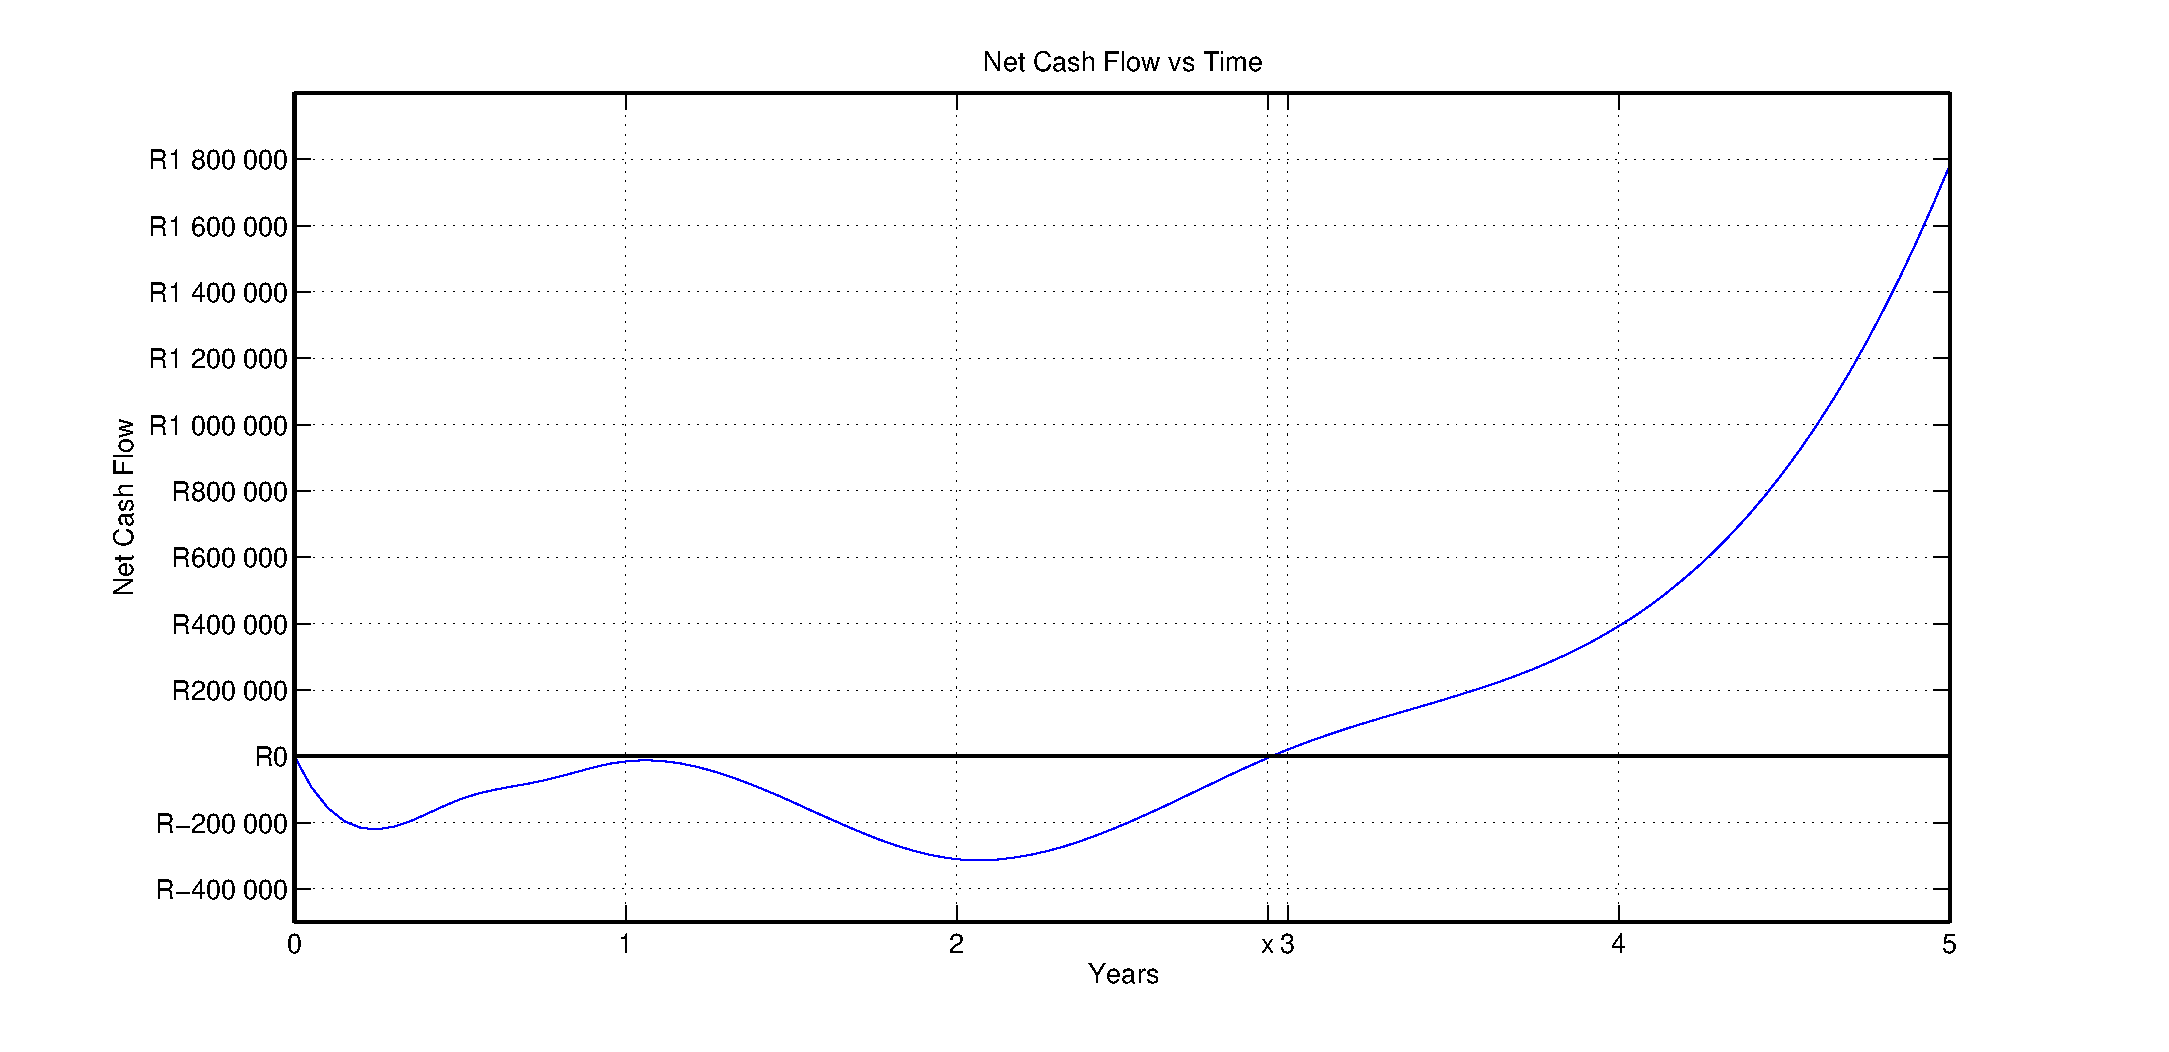
\includegraphics[width=0.9\textwidth]{images/cashflow_plot}
%\vskip10pt
\caption[Cash-flow plot]{Plot of cash flow in the business excluding debt and equity capital injections}
\label{fig:exam}
\end{figure}


\section*{Operations plan}
The Uvuka office location is likely to be In Longmeadow, Johannesburg. This will allow the business to have better contact with the Gauteng and Kwa-Zulu Natal customers that we plan to serve. It also offers a cost-effective rental compared to an equivalent premises in Cape Town.

Our five founding members consist of a combination of Mechatronic and Electrical \& Computer engineers, with each servicing a unique role on the Uvuka team. 

\cleardoublepage
\phantomsection
\addcontentsline{toc}{chapter}{Table of Contents}
\renewcommand{\contentsname}{Table of Contents} %change table of contents's name from 'contents' to 'table of contents'
\newpage %page break
\phantomsection %for some reason this gets the bookmarks to work

\tableofcontents



%\addcontentsline{toc}{chapter}{Section:} %add "table of contents" to the table of contents
\newpage %page break
\newpage

\cleardoublepage
\phantomsection
\addcontentsline{toc}{chapter}{List of Figures}
\listoffigures
\newpage

\pagenumbering{arabic}	%start the page numbering (and reset it to zero)
\chapter{Introduction}
%In South Africa, there were 4 500 road accidents which claimed the lives of more than 5 500 people between 2014 and 2015 \cite{EWNRoadDeaths}. Uvuka seeks to reduce the number of deaths on the road by providing a driver-monitoring device, which will set off alarms when a driver becomes drowsy and closes their eyes. This device is targeted at drivers who spend many hours on the road and are prone to fatigue. It can be used by individuals or by companies who own fleets of trucks, buses, or taxis. As this device will be permanently mounted inside the company's vehicles and will be linked to the main control room, the company will be able to monitor the drivers and receive alerts to make radio contact if a driver is becoming too drowsy to drive, thus ensuring their safety.


\section{Background}
In South Africa, there were 4500 road accidents which claimed the lives of more than 5500 people between 2014 and 2015 \cite{EWNRoadDeaths}. Around 25\% of these accidents were due to delayed reactions in fatigued drivers.

\section{Uvuka's Mission}
Uvuka seeks to reduce the number of deaths on the road by providing a driver-monitoring device, which will set off alarms when a driver becomes drowsy and closes their eyes or is distracted. This device is targeted at drivers who spend many hours on the road and are prone to fatigue. It can be used by individuals or by companies who own fleets of trucks, buses, or taxis. As this device will be permanently mounted inside the company's vehicles and will be linked to the main control room, the company will be able to monitor the drivers and receive alerts to make radio contact if a driver is becoming too drowsy to drive, thus ensuring their safety.

\section{Purpose of Business Plan}
This business plan lays out the progress made to date by our budding company, in order to secure investments that will enable Uvuka to continue to grow. It provides detail on the product, marketing strategy, financial plan, and business operations.

\section{Layout of Proposal}
The business plan begins by describing the product in detail. The marketing plan is then presented where the problem is dealt with in more detail and the target market as well as the competitors in this field are discussed. The finances of the company establish the required figures an projections including the operation time-line, expected costs, and cash flows. Lastly, the operations plan will describe the possible business office location, the manufacturing process, the production time-line, the team members, and how we plan to extend our business going forward.

\newpage 
\chapter{Product Description}
\section{Product Overview}
Uvuka seeks to reduce road accidents through intelligent monitoring of vehicle drivers. The product consists of a single device that mounts onto the dashboard of a vehicle, as seen in \cref{fig:Uvuka_casing_concept}. The basic working version of the product will have a camera pointing in the direction of the driver that focuses on the driver's face. The device will monitor the driver's eyes and detect if they close or begin to show signs of fatigue. If the eyes close for a set period of time (longer than the average blink), then the device assumes that the driver is beginning to fall asleep and takes appropriate measures to wake the driver up.

\begin{figure}[H]
\centering
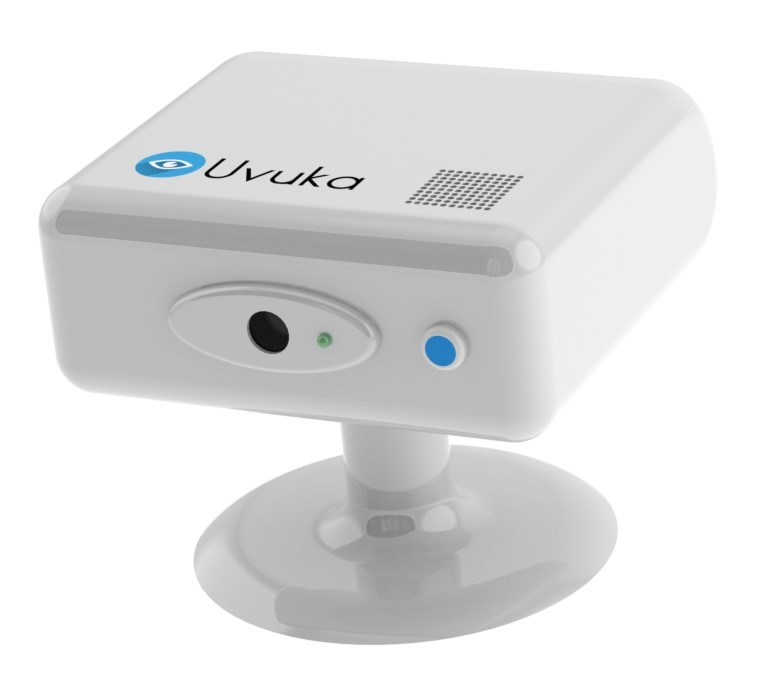
\includegraphics[width=0.8\textwidth]{images/Uvuka_casing_concept.JPG}
\vskip10pt
\caption{Conceptual design of Uvuka device rendered in SolidWorks}
\label{fig:Uvuka_casing_concept}
\end{figure}

Uvuka currently has the Uvuka Pro concept as the flagship product. Having a single product in these early stages allows the company to establish itself and focus resources on a particular device. An extended product range will eventually center around the same goal (keeping the driver awake while driving) but with different features present in different models. The first prototype produced will be the most elementary device, and once orders have been secured and units delivered, more advanced products can be developed and brought to market.

\section{Technical description of Uvuka}
\label{sec:Technical description of Uvuka}
The basic product consists of four main hardware components:
\begin{enumerate}
  \item \textit{Eye camera} - The eye camera faces the driver and provides a real-time video feed of their face, upon which algorithms can be performed. The camera is able to capture suitable low light footage for all driving conditions.
  \item \textit{Audio speaker} - The audio speaker is used to alert the driver. The speaker will play randomly generated tones that vary in frequency and duration. This prevents the driver from growing accustomed to the tones and thus will be more likely to wake him up \cite{Habituation}.
  \item \textit{Micro-controller and Inertial Navigation System} - The micro-controller needs to be powerful enough to perform real-time video processing. Eye-tracking and detection is done using OpenCV algorithms - these are free and open source video and image processing software algorithms. The micro-controller will also control the speaker and starts playing sounds when the driver begins to fall asleep \cite{OpenCV}. An Inertial Navigation System (INS) will include the necessary accelerometers, gyroscopes, and magnetometers to record the vehicle's dynamics and driver's handling of the vehicle.
  \item \textit{Power Supply} - The device can either be plugged into the standard 12 V cigarette plug, or it can be directly connected to the car power source for permanent mounts. The power is regulated to the correct voltage within the device, which will also include surge protection.
\end{enumerate}

The product has various modes of operation as seen in \cref{fig:DeviceFlowChart} below. The system defaults to the passive scanning mode where the device detects the driver's face and monitors eye movement. If the eye is determined to be closed, the device  enters a minor emergency state and assumes the driver's concentration has begun to wane. A brief sound is emitted to alert the driver. If this does not cause a satisfactory level of alertness, it assumes the driver is at risk of falling asleep and proceeds to take more drastic action. The action taken depends on the time the driver remains unresponsive and will vary from one type of device to the other.

\begin{figure}[H]
\centering
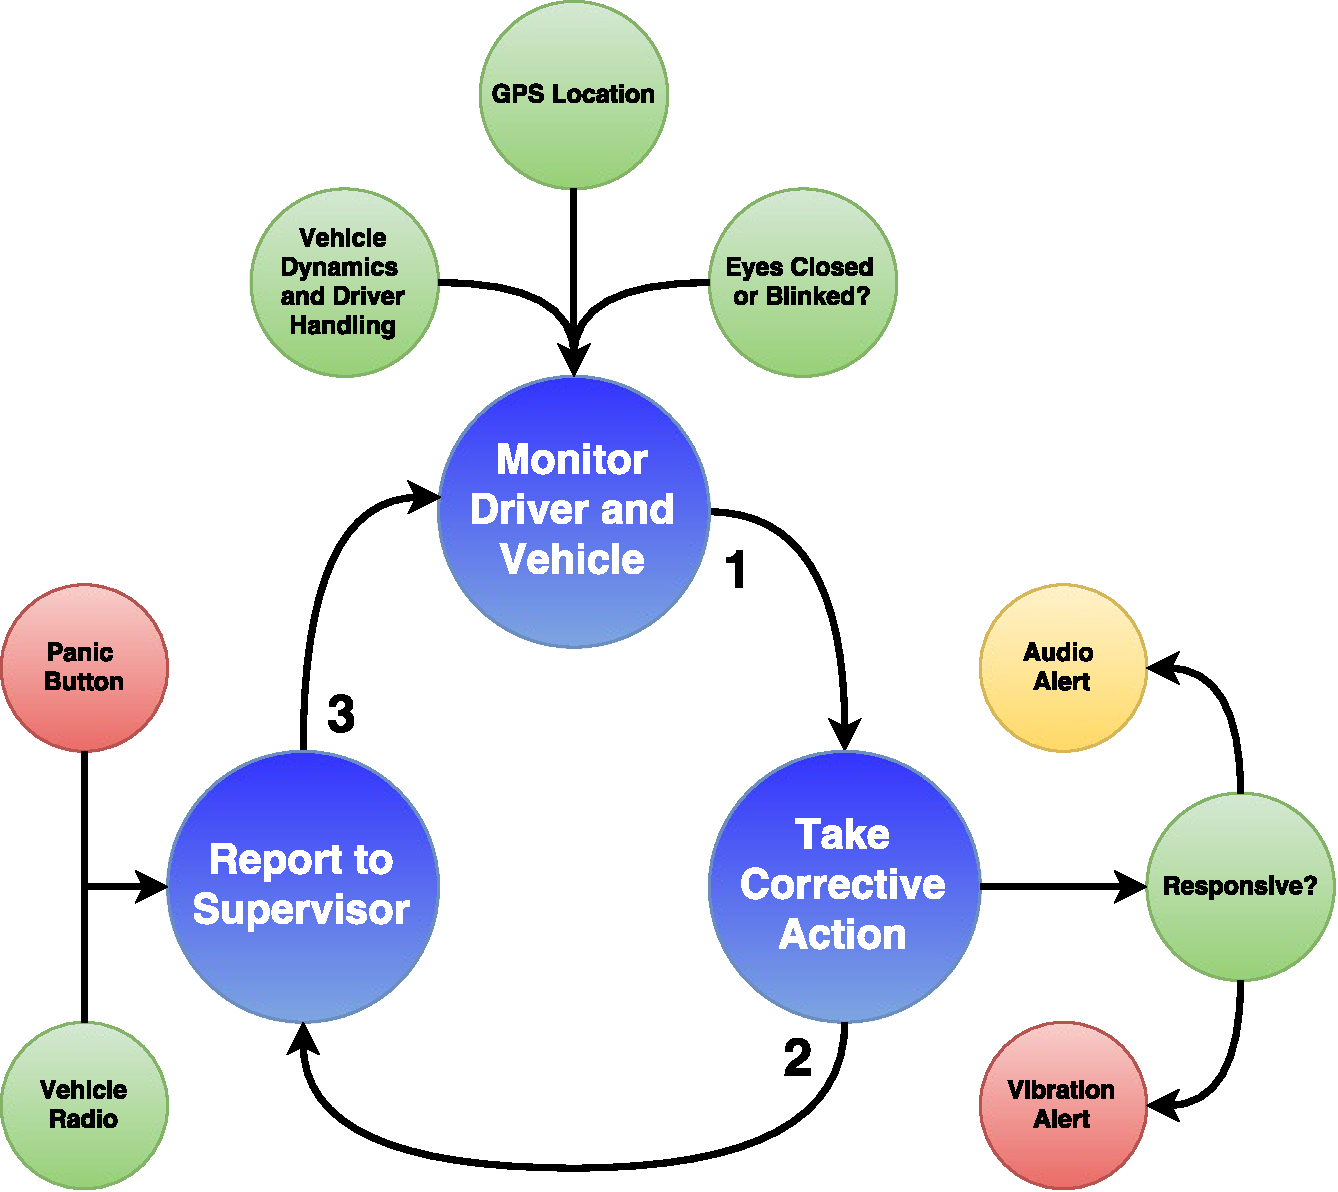
\includegraphics[width=1\textwidth]{images/NVP_Poster_Flowchart.pdf}
\vskip10pt
\caption[Device Operation Activity Diagram]{Process diagram of the device operation}
\label{fig:DeviceFlowChart}
\end{figure}

%TODO - BEN: talk about what is going on in this picture, and how it is an actual working system, not just something we did in paint. Although the colours kinda are.

\begin{figure}[H]
\centering
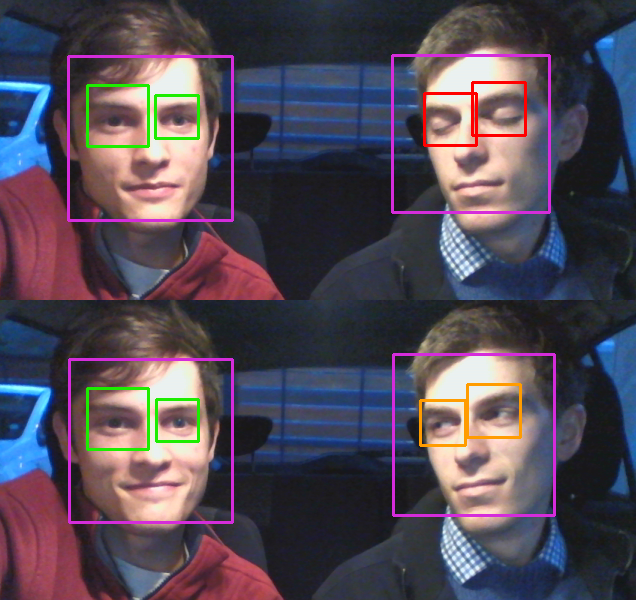
\includegraphics[width=1\textwidth]{images/ocv}
\vskip10pt
\caption[Optical feature recognition]{Optical feature recognition - responsive (green), unresponsive/distracted (orange) and closed (red) squares on eyes show proof of concept}
\label{fig:DeviceFlowChart}
\end{figure}

\section{Product Range}
The the Uvuka Pro explained in \cref{sec:Technical description of Uvuka} above is envisioned as being the initial market entry product that commercial customers will be able to order. This will be targeted at freight companies' truck drivers who require this device. As the business grows, the product range will be expanded based on consumer feedback and market research.

There are a number of other products and expansions planned:
\begin{itemize}
\item Uvuka Companion: This product is aimed at taxi operators and delivery drivers that are behind the wheel for extended periods of time. They are more likely to drive while tired or near exhausted (some taxi drivers can have shifts over 14 hours long \cite{taxiDriverHours}). In this case, sound may not be enough to wake them up. This product will have a strip attached to the steering wheel that will vibrate if the driver begins to fall asleep.
\item Uvuka Pro+: this product also incorporates the eye camera and vibrating steering wheel attachment. Additionally, it also has a second camera facing the road in front of the driver and a GPS unit to track the vehicle's location. All this data is recorded on an SD card. This system is aimed for long distance freight vehicles and allows fleet managers to monitor their drivers and vehicles through the INS data for quality and insurance purposes.
\end{itemize}

\section{Advantages of Uvuka over competitor products}
\label{sec:advantages}
Uvuka's devices will include unique features that allow them to perform several of the tasks currently performed by competing products. The primary difference in our innovative product is in our communications link between the driver and an external onlooker. This allows real-time monitoring that ensures the driver cannot simply ignore the device alerts or turn the device off without alerting the supervisor. Toyota and Seeing Machines are two companies that have developed devices which share certain similarities with our product. These are presented below.

Toyota have been implementing driver alertness technology in their luxury Toyota Crown vehicles since 2008. This allows the on-board computer to calculate how open the driver's upper and lower eyelids are as seen in \cref{fig:toyota_sensors}. They also include proximity sensors outside the vehicle to allow advanced preparation of brakes or airbags depending on the likelihood of a collision \cite{toyota}. 
\begin{figure}[H]
\centering
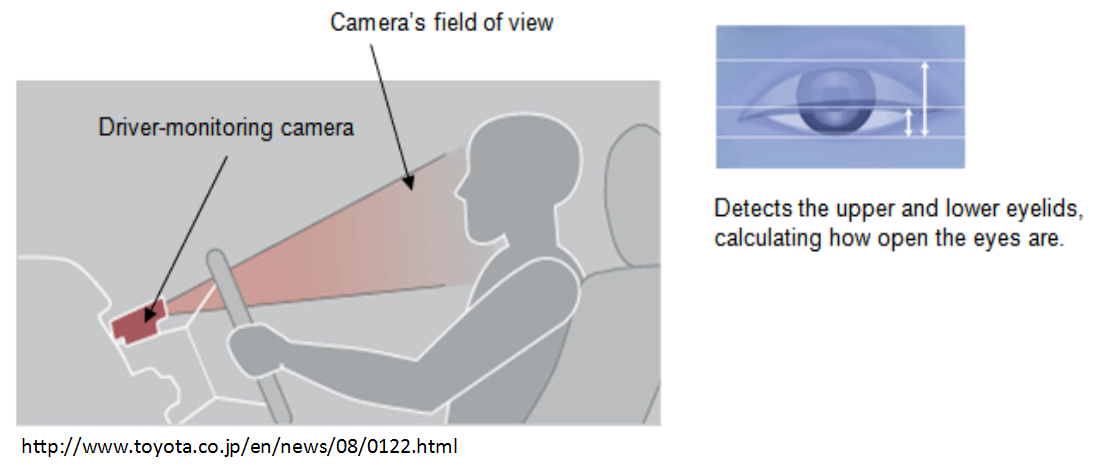
\includegraphics[width=0.9\textwidth]{images/toyota.PNG}
\vskip10pt
\caption[Toyota driver alertness system]{Toyota's driver alertness system tracks eyelids in real-time \cite{toyota}}
\label{fig:toyota_sensors}
\end{figure}
\pagebreak
Seeing Machines partnered with Intel, Land Rover, and Jaguar to integrate their technology into a Jaguar F-type at the 2015 Consumer Electronics Show. This further displays the relevance of this technology today internationally. A camera monitors the driver to determine the early signs of drowsiness or distraction in the form of eyelid closing as well as tilting of the head, a common indication that the driver is beginning to fall asleep. Warning signs are then given to the driver via the on-board touchscreen, in the form of audio and visual alerts \cite{sm_similarities}. A video still is shown in \cref{fig:sm_video} with a lighter circle in the centre showing the direction in which the driver is looking.
\begin{figure}[H]
\centering
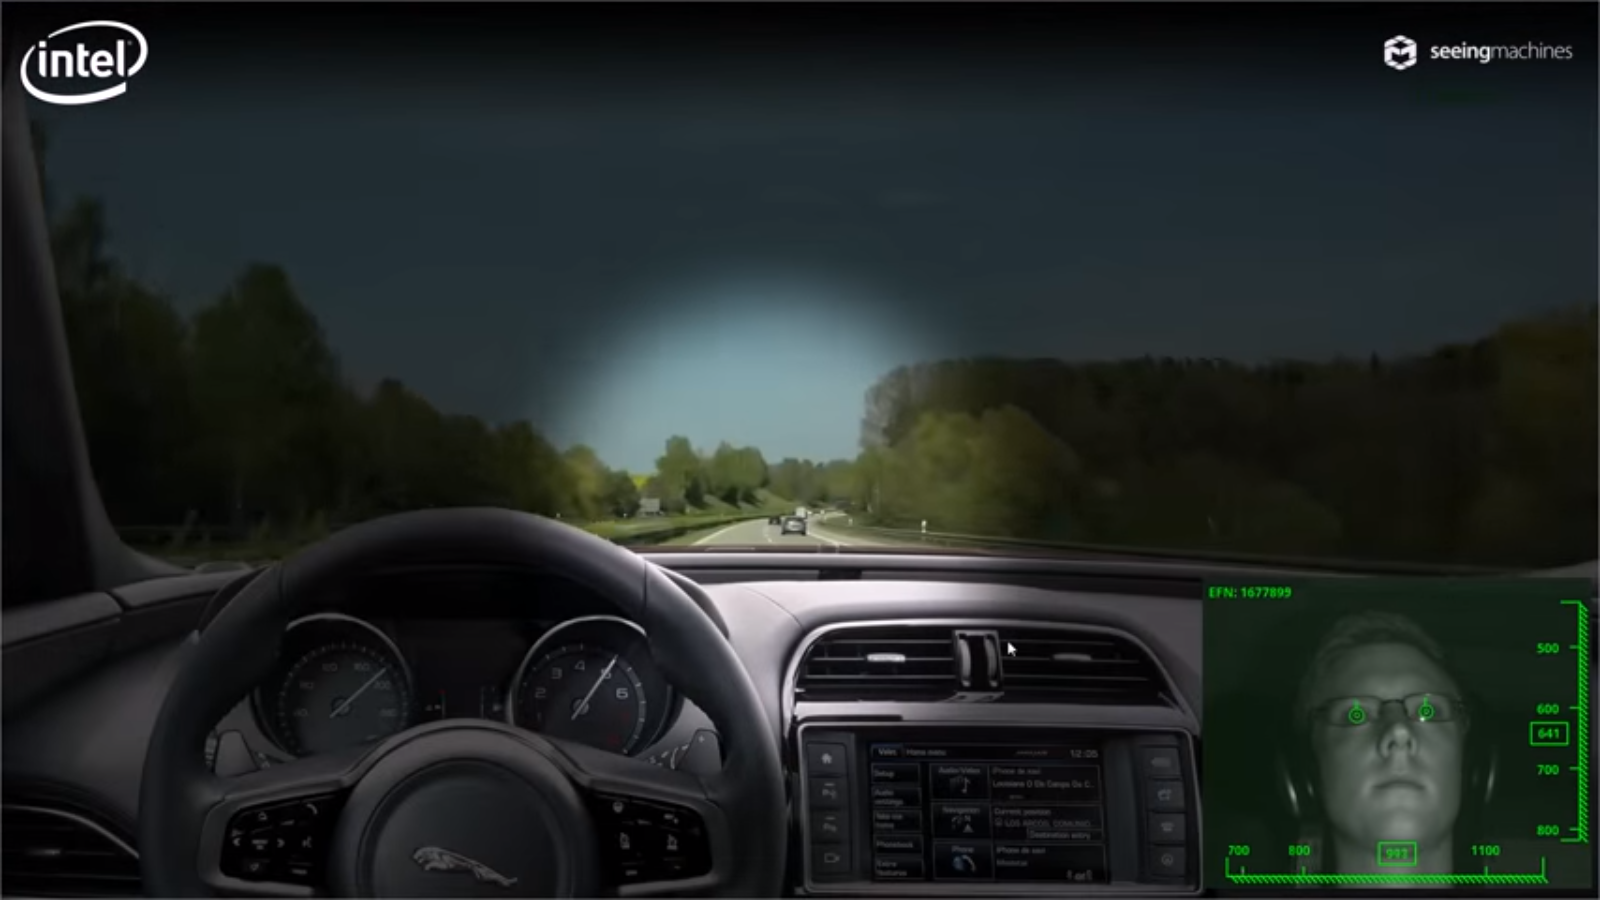
\includegraphics[width=0.8\textwidth]{images/seeingmachines.png}
\vskip10pt
\caption[Toyota driver alertness system]{Seeing Machines technology tracks driver's pupils to determine drowsiness or distractions and provide warnings \cite{sm_similarities}}
\label{fig:sm_video}
\end{figure}

\section{Product positioning}
The product will need to be versatile in order to cater for the needs of a number of different industries. The following sectors to be are considered:
\begin{itemize}
\item Heavy duty freight truck drivers
\item Bus drivers
\item Construction equipment operators (cranes, diggers, etc.)
\item Taxi drivers
\item Private use
\end{itemize}

\section{Intellectual Property and freedom of trade}
%Luke wants to do this section :P
%-Patent for the software/device that links camera to monitoring center.
%note: i'm just putting down words now, i've got no idea what i'm talking about

As briefly mentioned \cref{sec:advantages}, this drowsiness sensing technology has been around for a number of years. Uvuka, however, brings new ideas to the fold by incorporating fleet monitoring systems with a control center communications link - something that is yet to be made commercially available. It is for this reason that Uvuka applied for, and received their own patent on their communications link which alerts the control center of a driver who is showing signs of fatigue. This then allows the control center to check in on the driver and ensure their safety.

\newpage
\chapter{Marketing Plan}
\section{Problem background}
The harrowing death toll statistics on our country's roads motivated the company to engineer a product capable of making them a safer place for all \cite{EWNRoadDeaths}. South Africa's railway system is currently unable to support the needs of the growing economy. With 88\% of all freight being moved on the roads \cite{BDlive_freight}, many truck drivers are exposed daily to the risks of falling asleep at the wheel \cite{ArriveAliveDriverTiredness} and increase the risk of road accidents caused by fatigue \cite{News24TruckersSleeping}.

In addition, \cref{tab:deaths100thousand} shows that South Africa is significantly behind both developed and developing countries in the effort to curb road accident deaths, ranked \nth{36} in the world for number of road deaths per 100 000 inhabitants \cite{deathsPer100thousandStats}.


\begin{table}[htbp]
  \centering
  \caption{Indication of South Africa's road death crisis}
    \begin{tabular}{cc}
    \toprule
    \textbf{Region} & \textbf{Road deaths per 100 000 inhabitants} \\
    \midrule
    South Africa & 27.6 \\
    North America & 10.4 \\
    Australia & 5.6 \\
    Argentina & 12.0 \\
    Colombia & 12.0 \\
    Malaysia & 23.8 \\
    \bottomrule
    \end{tabular}%
  \label{tab:deaths100thousand}%
\end{table}%

To understand the regional road death statistics, the figures over the two-month festive season 2014/2015 in which 1 376 fatalities occurred are shown in \cref{fig:festiveSeason}. Each province experiences varying fatalities depending on its size and population density \cite{ProvincialFestiveStats}. Most notably, Gauteng and KwaZulu-Natal make up for a significant portion of the fatalities with 223 and 237 deaths respectively. Uvuka will seek to target customers operating in these two provinces specifically by setting up head offices in Johannesburg.

\begin{figure}[H]
\centering
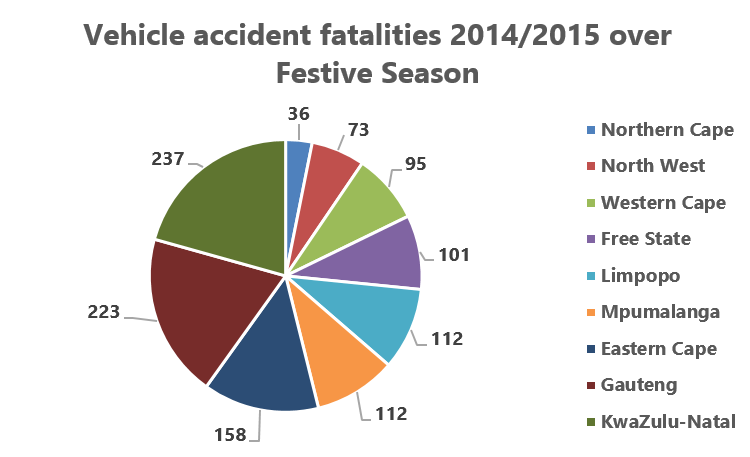
\includegraphics[width=1\textwidth]{images/provincial_fatalities.PNG}
\vskip10pt
\caption[Provincial fatalities for the period from 1 December 2014 to 7 January 2015]{Provincial fatalities for the period from 1 December 2014 to 7 January 2015}
\label{fig:festiveSeason}
\end{figure}

\section{Target market}
Freight companies are the primary customers that Uvuka will seek to cater for in the automotive industry. As outlined in the problem background, these companies are significantly more likely to require driver monitoring technology in the South African context as they work their long shifts on our nation's overcrowded roads.

In addition to the larger freight companies, smaller companies and couriers may also be interested in installing these devices. However, the more established enterprises are expected to make up the majority of our sales.

\section{Competitor product analysis}
\label{sec:competitoranalysis}
There are currently two primary international competitors producing a similar product. Seeing Machines, a company based in Australia, have developed a technology that tracks driver eyelid movement through computer vision algorithms \cite{SeeingMachinesWebsite}. They monitor the frequency and duration of blinking, as well as eyelid velocity. If the driver’s head begins to drop, an audio alarm is triggered and the seat vibrates. If they fall asleep again, a dispatcher is alerted and may make radio contact with the driver to check if they need a break. Seeing Machines has specifically worked with drivers that operate Caterpillar mining equipment \cite{SeeingMachinesWired}.

The second competitor company is Exeros, based in the United Kingdom \cite{Exeros}. Their product is targeted at businesses that operate a fleet of vehicles. When the driver begins to fall asleep, audio tones are sounded to attempt to wake them up. The devices they produce are able to be connected to an external GPS so that when an alarm is triggered, an outside individual can be notified of the occurrence and the location.

\section{Market strategy}
Once the context in which the device will operate is established, a market analysis will provide improved targeting of potential customers and insight into market trends. No South African competitors currently exist and so the company is expected to capture a significant portion of the market due to the product’s relative novelty and necessity.

\subsection{Initial market research}
Approximately three months will be set aside once the business has begun in order to conduct extensive research into the current market for this product. This will allow for better product positioning and ensure maximum impact of any targeted advertising. The following areas will need to be investigated:
\begin{itemize}
	\item \textit{How much will an Uvuka device cost to manufacture?} - manufacturing companies will need to be contacted before the prototyping process in order to accurately estimate the costs involved.
	\item \textit{What are customers prepared to pay for a driver monitoring device?} - truck companies and commercial drivers will be asked what their expectations are for the products features and its price.
	\item \textit{How many Uvuka devices will be required in order to curb road accident deaths in South Africa?} - South African road accident statistics will need to be further analysed in order to provide a reasonably accurate estimate of this figure.
	\item \textit{Which companies should the business approach for the first stage of product roll-out?} - an investigation into which companies travel in the more dangerous provinces will provide further insight.
	\item \textit{How will commercial drivers react to being monitored constantly?} - drivers will need to be interviewed in order to obtain their feedback. This way Uvuka will be able to position itself as a tool that saves lives, and not something that is there to spy on employees.
\end{itemize}

 \section{SWOT analysis}
A SWOT analysis is a common market research tool that analyses the Strengths, Weaknesses, Opportunities and Threats faced by a particular company. This is presented below in terms of internal and external origin:
\pagebreak
\subsection{Internal origin}
\subsubsection{Strengths}
\vskip8pt
\begin{itemize}
\item compact size, non-intrusive when mounted on the dashboard
\item relatively low cost to manufacture as well as selling price
\item functionality (GPS, integrated sensors, camera, alerts)
\item outsourced manufacturing of components with on-site assembly to control quality
\item initial small-scale business structure enables rapid adjustments and fine tuning
\item low power consumption while in use
\item potential to add features (road-facing camera)
\end{itemize}
\vskip15pt
\subsubsection{Weaknesses}
\vskip8pt
\begin{itemize}
\item people often dislike being monitored
\item the device may be seen as an intrusion
\item devices are at risk of being tampered with by commercial drivers
\item success relies on established companies to try something new from a small start-up that is yet to establish a reputation (reluctant customers)
\item legal implications if vehicle crashes due to driver fatigue despite Uvuka monitoring being installed and in use
\end{itemize}
\vskip15pt
\subsection{External origin}
\subsubsection{Opportunities}
\vskip8pt
\begin{itemize}
\item no immediate local competitors
\item the market could be dominated quickly
\item growing economy requires more trucks on the road and could allow increased sales
\item companies are looking to keep their drivers and loads safer
\item government is constantly seeking to reduce death toll on roads
\item expansion into Southern Africa once established nationally
\end{itemize}

\vskip15pt
\subsubsection{Threats}
\vskip8pt
\begin{itemize}
\item devices may be easy to replicate and so new competition could catch up quickly
\item employers could misuse devices to spy on employees' activity while driving
\item risk of theft from vehicle as device is very visibly mounted onto dashboard
\end{itemize}
\vskip15pt

\section{Uvuka product name and logo}
``Uvuka" literally means ``wake up" in Zulu. Other variations of the word are ``vuka" (get up) or ``uvukile" (to wake up), but it was felt that ``Uvuka" was the most suitable of these derivatives. This name gives an indication of the urgency in waking up, as well as a direct link to the South African origins of the company.

In order to convey the product's purpose and the company's values, a logo was designed as seen in \cref{fig:uvuka_logo}. This seeks to motivate the product to potential investors and customers as a device that keeps an eye open in order to ensure your safety or the safety of your employees on the roads.

\begin{figure}[H]
\centering
\includegraphics[width=0.7\textwidth]{images/uvuka_logo_ben}
\vskip10pt
\caption[The Uvuka logo]{The Uvuka logo}
\label{fig:uvuka_logo}
\end{figure}

\section{Strategic partnerships}
In order to gain more traction in the market, Uvuka will seek to partner with the Automobile Association (AA) in South Africa. This will allow us to gain accreditation and influence within the automotive sector which is always seeking new ways to improve safety on the nation's roads.

In addition to the AA, a partnership with an insurance company like Santam or Mutual \& Federal would be beneficial. Our devices would be able to reduce the insurance risk on the road and allow the insurer to offer a lower premium on their clients' policies that cover vehicles fitted with Uvuka hardware.

\newpage

\chapter{Finances}

\section{Time-line of Operation}
In order to accurately estimate the finances of the company, a timeline of business operations is constructed:

{\bfseries \nth{1} Quarter of Operations}
\begin{itemize}
\item An initial amount of R250 000 is injected by the owners into the business.
\item All five owners start working at the same time, each for a salary of R10 000 a month.
\item All owners are working from their private residences for the first quarter and as such no rent needs to be paid.
\item The prototyping stage begins - this R50 000 is used to buy and manufacture the components.
\item R20 000 is used to purchase a high-end desktop PC to run simulations as well as a printer.
\end{itemize}

{\bfseries \nth{2} Quarter of Operations}
\begin{itemize}
\item R500 000 is invested into the company by external investors.
\item Office space is rented for approximately R14 000 a month (including utilities).
\item Prototyping is completed after the fifth month.
\item Products are manufactured and sold in the sixth month of operation.
\end{itemize}

{\bfseries \nth{3} Quarter of Operations}
\begin{itemize}
\item A salesperson is hired at the start of the third quarter for R10 000 a month.
\end{itemize}

{\bfseries \nth{4} Quarter of Operations}
\begin{itemize}
\item The fourth quarter is spent selling the product and expanding the customer base. No new operating expenses are incurred here.
\end{itemize}

{\bfseries \nth{2} Year of Operations}
\begin{itemize}
\item Manufacturing is increased in the second year. A loan of R500 000 is taken out from a bank at an interest rate of 10\% per annum p.a. to be paid over ten years. 
\item A technician is hired on a salary of R10 000 a month.
\item The 5 original owners have their salary increased to R11 000 a month.
\item A part time cleaner is hired to clean the office for R5 000 a month.
\end{itemize}
\pagebreak
{\bfseries \nth{3} Year of Operations}
\begin{itemize}
\item Product marketing to general public begins. Direct sales to freight companies are continued alongside private sales. Advertising is used to increase brand and product presence.
\item Owners have their salary increased to R13 000 a month.
\end{itemize}

{\bfseries \nth{4} Year of Operations}
\begin{itemize}
\item All staff members receive a salary increase of 6\%.
\item One more technician is recruited. The new recruit's salary matches the other technicians' new salary.
\end{itemize}

{\bfseries \nth{5} Year of Operations}
\begin{itemize}
\item The business is on track to reach a yearly turnover of R5 000 000 by the end of this year. Options will be explored to manufacture products in-house and in larger volumes.
\end{itemize}

There are some additional costs that will be included in the expenses:
\begin{itemize}
\item Office supplies - these will be part of capital expenditure.
\item Rent and Utilities Payment - this is all included in the rent cost section of the balance sheet. The current rent cost is budgeted to be R14 000 per month. The property cost is R65/m$^2$. R10 000 of this is used to pay the rent (approximately 150 m$^2$) and the rest goes to utilities and maintenance cost. This amount is expected to increase with inflation. 
\end{itemize}

\section{Expected Product Cost and Markup}
Estimations for the number of products produced and sold are made in \cref{tab:ProductSales}. Very few products are produced in the first year of operation as a portion of the year is spent developing the product and making an initial entry into the market. The product materials and manufacturing cost is the largest expense for the business by far. This table assumes that when additional products are released, they will sell for the same price as the basic version. This is therefore a conservative estimate as later additions could potentially be sold at a higher markup while still costing approximately the same amount to manufacture.

The values listed are excluding VAT which must be included when selling to the customer. The cost to assemble the raw materials and have them manufactured is shown in \cref{tab:productCost}. The total cost of product is calculated using the raw material and manufacturing costs but also includes the labour costs (technicians' salaries). This price is increased every year with inflation. 

The markup of the product is calculated to ensure that we have made a profit, while still ensuring that our product is not too expensive so as to leave Uvuka exposed to cheaper competing alternatives.

\begin{table}[htbp]
  \centering
  \caption{Summary of Product Costs}
    \begin{tabular}{p{0.12\linewidth}p{0.11\linewidth}p{0.11\linewidth}p{0.12\linewidth}p{0.12\linewidth}p{0.12\linewidth}p{0.12\linewidth}}
    \toprule
    \raggedright{Year of Operation} & Quantity Produced & Quantity Sold & Selling Price & Raw Materials Cost & \raggedright{Total Cost Price} & Contribution \\
    \midrule
    1     & 220   & 200   & R 5 500.00 & R 3 044.00 & R 3 044.00 & R 2 456.00 \\
    2     & 440   & 400   & R 5 830.00 & R 3 226.64 & R 3 499.37 & R 2 330.63 \\
    3     & 740   & 650   & R 6 179.80 & R 3 420.24 & R 3 598.62 & R 2 581.18 \\
    4     & 850   & 800   & R 6 550.59 & R 3 625.45 & R 3 954.68 & R 2 595.91 \\
    5     & 1300  & 1250  & R 6 943.62 & R 3 842.98 & R 4 071.16 & R 2 872.47 \\
    \bottomrule
    \end{tabular}%
  \label{tab:ProductSales}%
\end{table}%

The current production estimates assume that there will be a surplus of units to sell for the next year of operation. From the above predictions, the total amount spent on manufacturing, cost of goods sold (COGS), and gross profit are calculated as shown in \cref{tab:GrossProfit}. 

% Table generated by Excel2LaTeX from sheet 'Sheet1'
\begin{table}[htbp]
  \centering
  \caption{Table showing gross profit of the business}
    \begin{tabular}{rrrr}
    \toprule
    Year of operation & Manufacturing Cost & COGS  & Gross Profit \\
    \midrule
    1     & R 669 680.00 & R 608 800.00 & R 491 200.00 \\
    2     & R 1 539 721.60 & R 1 399 746.91 & R 932 253.09 \\
    3     & R 2 662 976.42 & R 2 339 100.91 & R 1 677 769.09 \\
    4     & R 3 361 474.80 & R 3 163 740.99 & R 2 076 729.41 \\
    5     & R 5 292 504.23 & R 5 088 946.37 & R 3 590 582.73 \\
    \bottomrule
    \end{tabular}%
  \label{tab:GrossProfit}%
\end{table}%

It can be seen that Uvuka aims to greatly increases its gross profit over the first five years of operation. 

\section{Tax}

Uvuka will be required to pay tax. Vat is 14\% of the price on products sold and this value has already been removed before the information was entered into the cash flow and income statements. It will therefore not be dealt with elsewhere in this proposal.

The other tax that needs to be dealt with is income tax, at a rate of 28\% on the profits of the business. This value has been factored into the cash flow statement based on results calculated in the income statement.

\section{Employee Cost Breakdown}
Salaries are the second highest cost to the business. The salary breakdown is shown in \cref{tab:salaries}. The founders start off with a very low salary which increases proportionally with business growth. Only a single salesperson is needed as it is assumed the founders will also take part in product sales. While the founders have very little sales experience, they will work closely with the salesperson initially in order to gain insight into the required skills and techniques.

Only two technicians are required despite the higher volumes of monthly production. This is because manufacturing of most of the product components will be outsourced so the technicians will only be required for final product assembly and inspection. Furthermore, all the founders are trained engineers and will be more than capable of assisting with this work.

While initially the founders are paid a lower than average wage for an engineer, the salaries of the sales people and the technicians are relatively competitive. These wages will increase with inflation and the founders salaries could potentially be increased to industry norms once the business is turning a large enough profit.

% This table can be found in the cashflow statement
\begin{table}[htbp]
  \centering
  \caption{Table showing the salaries paid to employees}
    \begin{tabular}{p{0.14\linewidth}p{0.14\linewidth}p{0.14\linewidth}p{0.14\linewidth}p{0.14\linewidth}p{0.14\linewidth}}
    \toprule
    Salaries & Year 1 & Year 2 & Year 3 & Year 4 & Year 5 \\
    \midrule
    \raggedright{Each Initial Founder} & R 10 000 & R 11 000 & R 13 000 & R 13 780 & R 14 606 \\
    Salesperson & R 10 000 & R 10 000 & R 11 000 & R 11 660 & R 12 359 \\
    Technician 1 &       & R 10 000 & R 11 000 & R 11 660 & R 12 359 \\
    Technician 2 &       &       &       & R 11 660 & R 12 359 \\
    \raggedright{Part Time Cleaner}&       & R 5 000 & R 5 500 & R 5 830 & R 6 179 \\
    \midrule
    \raggedright{Total over Year} & R 660 000 & R 960 000 & R 1 110 000 & R 1 316 520 & R 1 395 511 \\
    \bottomrule
    \end{tabular}%
  \label{tab:salaries}%
\end{table}%

\section{Cash Flow Statement}
Based on the information outlined in the above sections, a cash flow statement for the first five years of business is created. A plot of the cash in the business is shown in \cref{fig:cashflowplot}. The actual statement is shown in \cref{fig:CashFlowStatement_horizontal}. The projected break-even point is within three years of operation. It can be seen that once the company breaks even, the cash-flow income grows at a rapid rate.

The first year of operation does not require as much capital as the second year as most of the first year is spent developing the product. Furthermore, when the product is developed, it does not require a large capital investment to manufacture it as this process can be outsourced. The rest of the first year is spent making initial forays into the market, finding initial customers and training the founders in sales. Once the second year of operation begins, more staff are hired and more products are manufactured, thus resulting in more expenses as overheads increase. These overheads eventually help the company break even and make a large profit after the break even point is reached.

\begin{figure}[H]
\centering
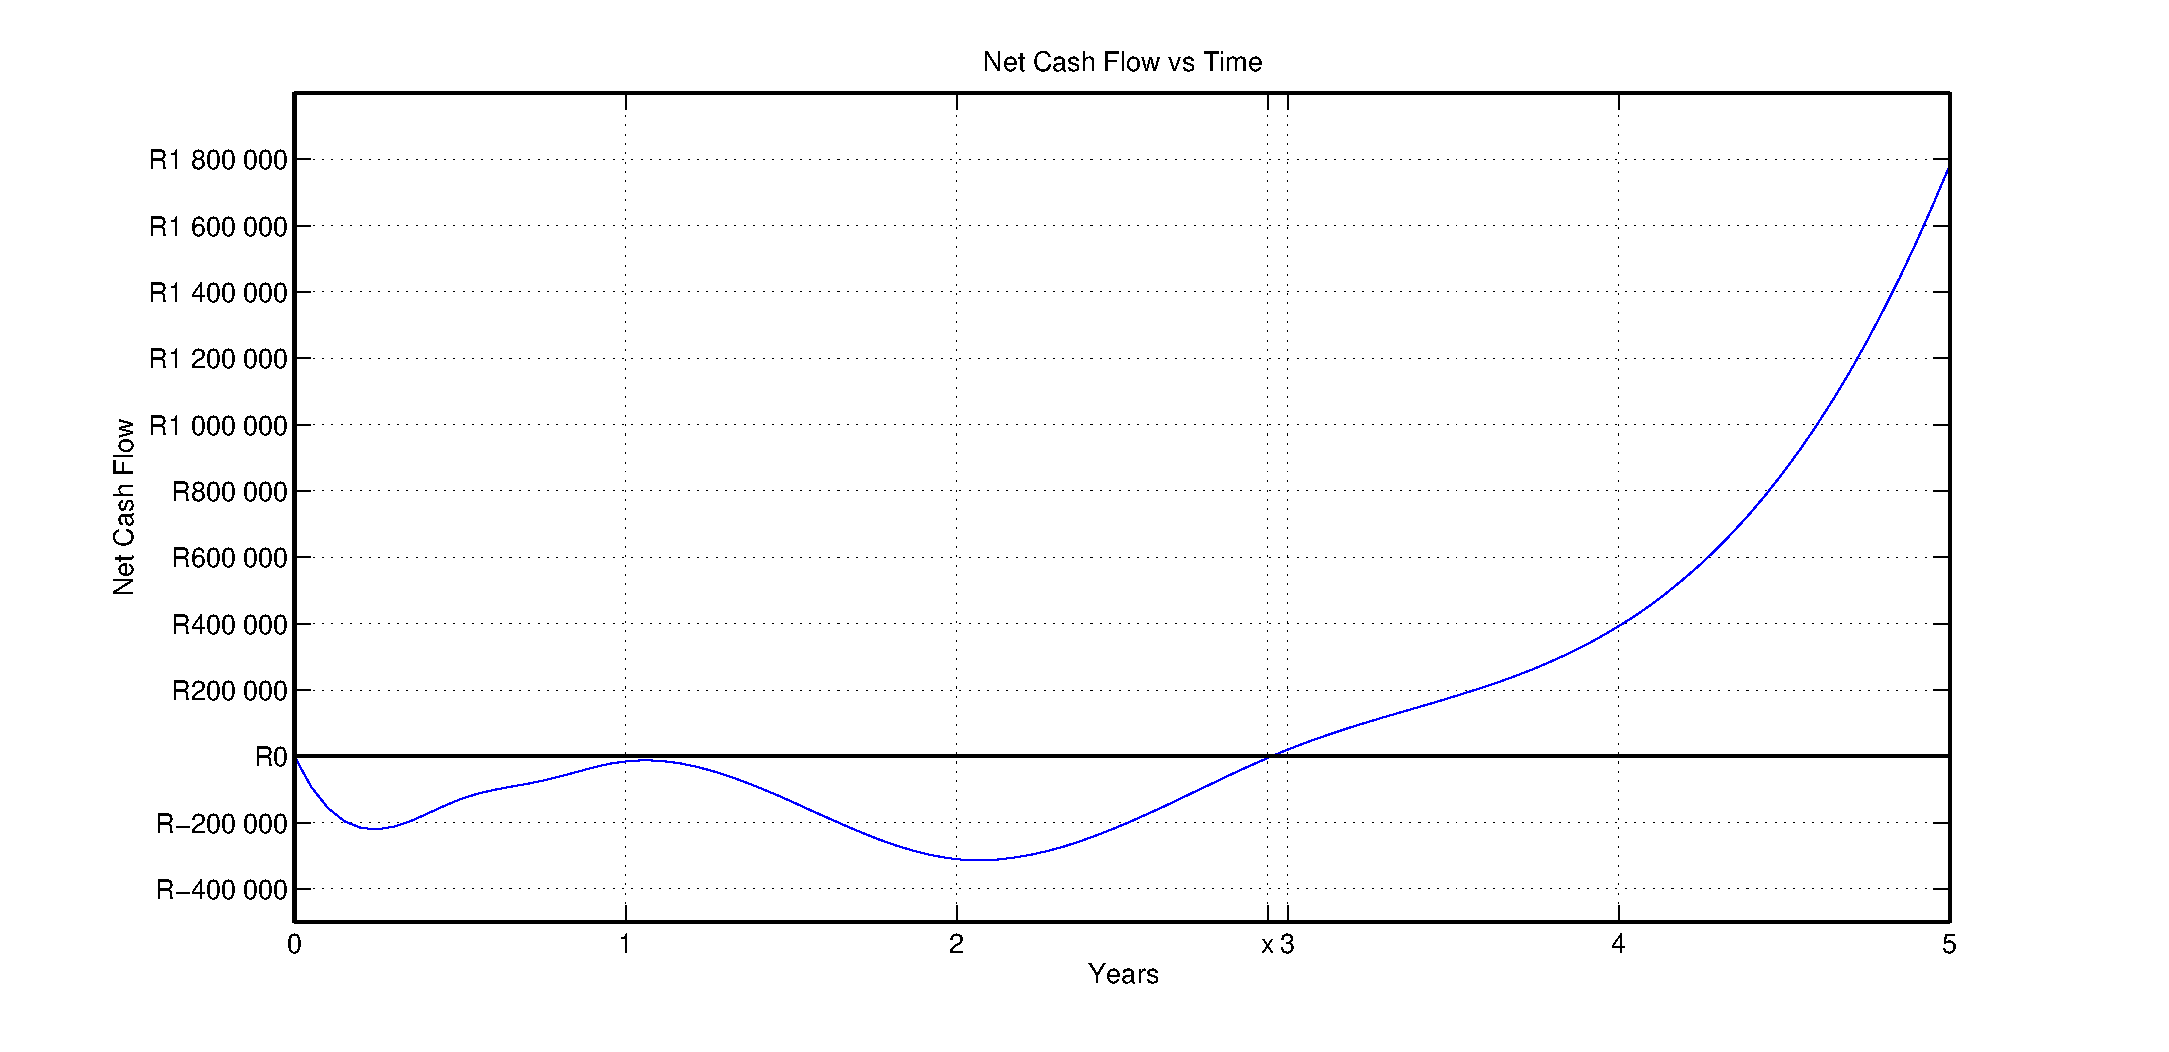
\includegraphics[width=1\textwidth]{images/cashflow_plot}
\vskip10pt
\caption[Cash-flow plot]{Plot of cash flow in the business excluding debt and equity capital injections}
\label{fig:cashflowplot}
\end{figure}

\newpage
\thispagestyle{plain}
\begin{landscape}
  \begin{figure}[H]
    \centering
    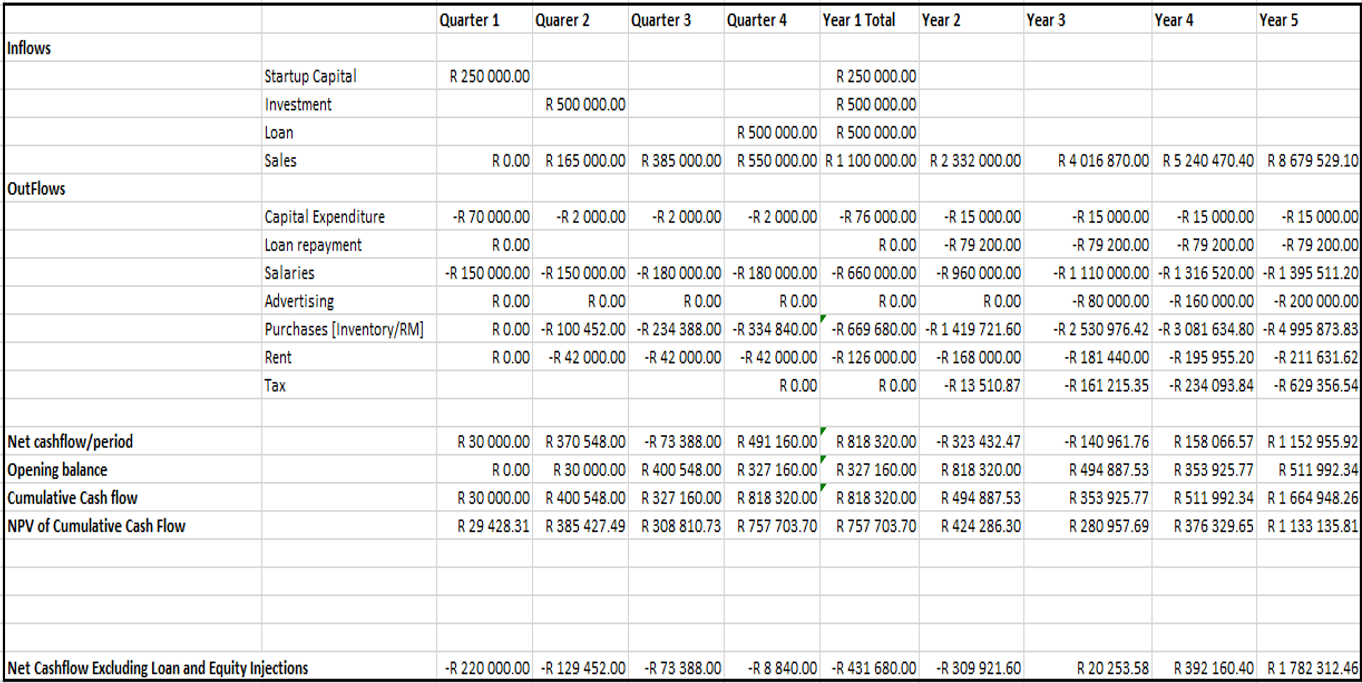
\includegraphics[width=1.5\textwidth]{images/CashFlowStatement_horizontal}
    \vskip10pt
    \caption[Uvuka Cash-Flow Statement]{Uvuka Cash-flow Statement}
    \label{fig:CashFlowStatement_horizontal}
  \end{figure}
\end{landscape}
\newpage


\section{Income Statement}

An income statement was drawn up for the first five years of operation from the cash flow statement. This statement is shown in \cref{fig:IncomeStatement} below. A strategy for accepting money on credit has not been discussed, thus the only sources of income come from the cash flow statement. 

  \begin{figure}[H]
    \centering
    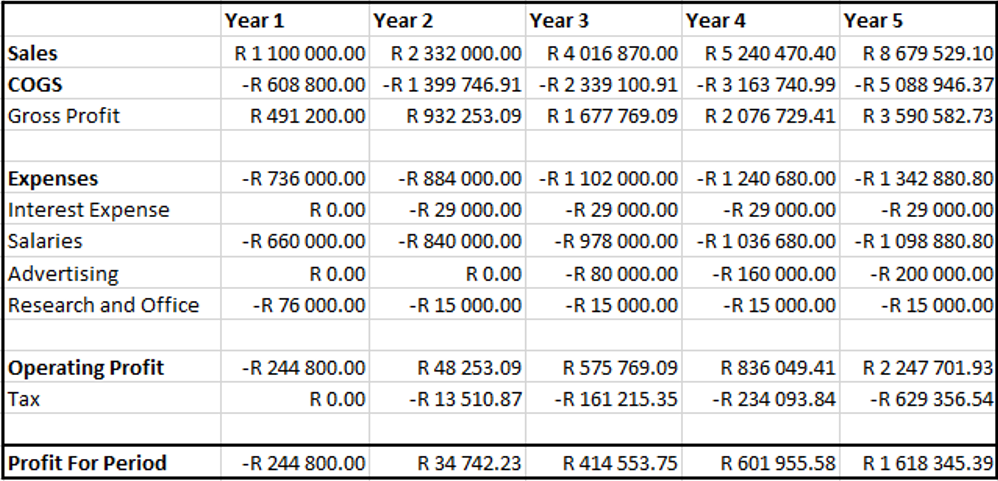
\includegraphics[width=1\textwidth]{images/IncomeStatement}
    \vskip10pt
    \caption[Uvuka Income Statement]{Uvuka Income Statement}
    \label{fig:IncomeStatement}
  \end{figure}

A loss is made in the first year of operations for a number of reasons:
  \begin{enumerate}
        \item \textit{Small Customer base} - in the first year of operations the Uvuka team is making its first forays into the market. No strategic partnerships have been formed and no customer base has been established. Over the years of operation this base will be expanded which allows the company to turn a profit in the future.
        \item \textit{Product development stage} - the product starts being sold mid-way through the year and so not enough of it will be sold to cover expenses.
        \item \textit{Founders are still being trained in sales} - the founders are still learning how to sell the product thus they will not sell as many as a fully-trained salesman could.
        \end{enumerate}
        
As the company continues to grow, it will begin to turn a profit. After 5 years the income far outweighs the expenses.

\pagebreak
\section{Balance Sheet}

Using the Cash-flow statement in \cref{fig:CashFlowStatement_horizontal} and the Income statement in \cref{fig:IncomeStatement}, a balance sheet is drawn up for the first five years of operation. This balance sheet is shown in \cref{fig:BalanceSheet} below. A few conclusions can be drawn from this balance sheet:
\begin{itemize}
	\item \textit{Few initial fixed assets} - Uvuka does not have many fixed assets. The founders use their own personal computers which reduces start-up costs. The property is rented instead of bought, and the product manufacturing is outsourced which eliminates the need to purchase expensive manufacturing equipment.  
    \item \textit{After 5 years Uvuka has large quantities of cash assets} - while Uvuka does not have many fixed assets by year five, it will have a large cash reserve. This will allow the company to withstand any unexpected crisis. Furthermore, these cash reserves can be used to expand the business or exploit opportunities that are discovered. This is a major strength
    \item \textit{Overall assets in the business decrease in the second year of operation} - the business spends a large portion of its funds in the second year on salaries as it continues to build up its customer base. The money in the business is not converted into other assets. Once the third year of operation is finished, the business assets are again increasing.
    
\end{itemize}

\begin{figure}[H]
    \centering
    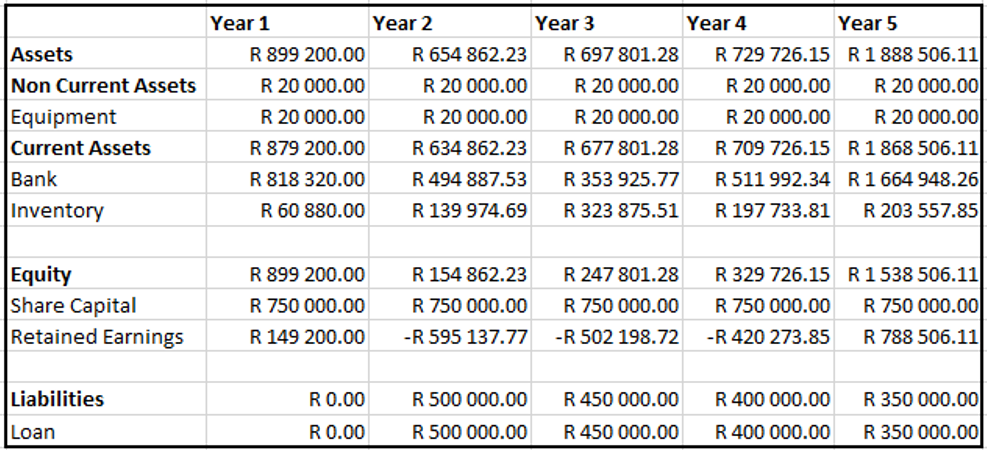
\includegraphics[width=1\textwidth]{images/BalanceSheet}
    \vskip10pt
    \caption[Uvuka Balance Sheet]{Uvuka Balance Sheet}
    \label{fig:BalanceSheet}
\end{figure}


\newpage

\chapter{Operations Plan}
\section{Business location}
As mentioned earlier in the Marketing Plan, our head office will be set up in Johannesburg. This provides us convenient access to the freight companies that make up our target market. In addition, we will be nearer to suppliers and are able to find a location with a lower rent than an equivalent setup in Cape Town.

This office space in Longmeadow (see \cref{fig:map}) is available for R65/m$^2$ and could provide the location Uvuka needs to grow as a new business. Its relatively low rental also allows the company to steward finances into areas of the business that will be more important for growth. The building, as shown in \cref{fig:offices}, appears to have suitable parking and security.

\begin{figure}[H]
\centering
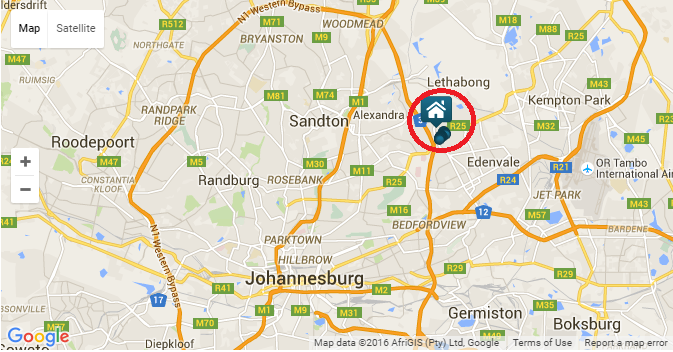
\includegraphics[width=0.75\textwidth]{images/offices_map.PNG}
\vskip10pt
\caption[Map showing potential office location in Longmeadow, north of Johannesburg]{Map showing potential office location in Longmeadow, Johannesburg}
\label{fig:map}
\end{figure}

\begin{figure}[H]
\centering
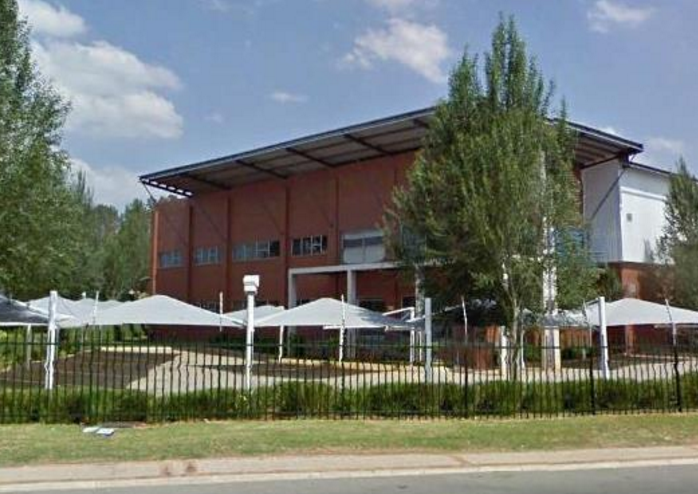
\includegraphics[width=0.55\textwidth]{images/offices_building.PNG}
\vskip10pt
\caption[Potential offices for Uvuka]{Potential offices for Uvuka that are available and suit our current business size with room for expansion}
\label{fig:offices}
\end{figure}

\section{Production and manufacturing}
%\textit{Ben do this bit :P Talk about how we will make the parts elsewhere, and then assemble it ourselves or whatever we are doing, also about how making it in-house will improve quality control and allow us to change things quicker than if we had to go through a whole supply chain, that kind of thing.}
%include risk management stuff associated with manufacturing here?
\subsection{Component Sourcing}
Mouser Electronics has a convenient online component database. They have a wide range of components and import directly to Cape Town. 

All components were sourced from Mouser in order to reduce the risk of importing from unknown sources in the early stages of the company - in future a reliable connection could be established in Asia where these components can be bought directly from the suppliers thus reducing the cost of production. 

\Cref{tab:productCost} provides a breakdown of the component costs and source, as well as the manufacturing methods and their estimated cost. These costs are conservative and are likely to be less when bulk discounted pricing is taken into account. The cost price of the Uvuka Pro system is calculated at R3 044.11. 

\begin{table}[htbp]
  \centering
  \caption{Table Showing the cost of all the components of the product}
    \begin{tabular}{LLLL}
    \toprule
    \textbf{Item} & \textbf{Component} & \textbf{Unit Cost} & \textbf{Source} \\
    \midrule
    \multirow{2}[2]{*}{GPS Module} & \multirow{2}[2]{*}{GPS UART Module} & \multirow{2}[2]{*}{R 218.94} & Mouser:  \\
          &       &       & 963-GYSFFMAXB  \\
    GSM Module & SIMCOM SIM900 GSM/GPRS Module & R 250 & SIMCOM \\
    Camera Module & OmniVision OV9712 IMAGE SENSOR MODULE & R 432.35 & Mouser: 931-LI-OV9712-FF-65  \\
    Embedded Linux System & Olimex A13 & R 992.82 & Mouser: 909-A13OLINUXINOMICR \\
    Miscellaneous  & Passive components & R 500 & Mouser \\
    PCB Manufacturing & PCB, Part Placement & R 250 & Zyteq Technologies \\
    Enclosure Manufacturing & 3D printing and injection moulding & R 300 & Skeg Product Development \\
    Product Assembly &       & R 100 & Uvuka \\

    \textbf{Total:} &       & R 3 044.11 &  \\
    \bottomrule
    \end{tabular}%
  \label{tab:productCost}%
\end{table}%

\newpage
\subsection{PCB Manufacturing}
The PCB manufacturing will be outsourced to Zyteq industries who have a PCB production and assembly line locally in Cape Town - this will allow rapid prototyping and quality control in the early stages of the company.

\subsection{Enclosure Manufacturing}
Initially 3D printing and subsequent injection moulding will be completed by Skeg product development in Cape Town, after which the process will be outsourced overseas to reduce production costs. 

\section{Production Timeline/ Schedule}
\begin{figure}[H]
\centering
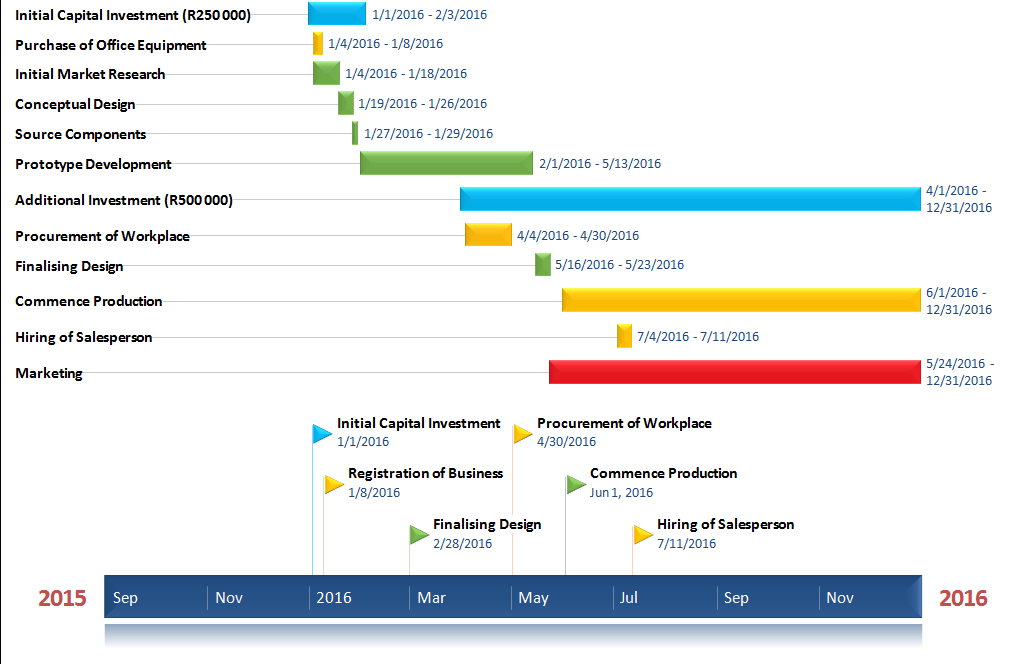
\includegraphics[width=1\textwidth]{Gantt_2016.PNG}
\vskip10pt
\caption[Gannt Chart of the first year of operations of Uvuka]{Gannt Chart of the first year of operations of Uvuka}
\label{fig:Gantt Chart 1}
\end{figure}


\section{Staff and team expansion} 

The current team consists of five founders:
\subsection{Munawwar Tayob - The big boss}
Munawwar holds a BSc. (Eng) in Mechatronics from the University of Cape Town. She......

\subsection{Benjamin Scholtz - Product Development}
Benjamin obtained his BSc. (Eng) in Mechatronics from the University of Cape Town. His interest in product development came from his months of experience working at the local product development company ManMakeMachine where he adopted the "Ideate, Prototype, Engineer" product development mindset. His work on a wide range of product development projects brings the broad perspective needed to make this company a success.  

\subsection{Roberto Aldera - Marketing}
Roberto obtained his BSc. (Eng) in Mechatronics from the University of Cape Town. His interest in market research and data analysis combines with an engineering mindset to better position Uvuka in the market.

\subsection{Gareth Callanan - Finances}
Gareth received his BSc. (Eng) in Electrical and Computer Engineering from the University of Cape Town in 2016. His engineering interests are in control engineering and hardware acceleration. Furthermore he has done a number of university accounting courses and takes a keen interest in all things financial. 

\subsection{Luke Goemans - Operations and Future Development}
Luke is an avid entrepreneur, with interests in system design, optimization, and a far-reaching vision. He obtained his BSc. (Eng) in Mechatronics from UCT, and his interests are applied within the Operations and Future Development section of Uvuka to stay abreast of the current developments and ensure that the company is always relevant to the market.

\subsection{Future Hires}

As Uvuka expands, it will be necessary to increase the number of team members hired. 

When the product first goes to the market, a salesman will be hired. This salesman must be able to both sell The product and help the five founders perfect their sales technique. In this way, the founders can also assist in selling the product and thus alleviate the need to hire more salespeople.

Uvuka will need to also start hiring technicians to help assemble and troubleshoot the product once production reaches high enough levels. These technicians will assemble the product from the delivered component parts, conduct quality checks as well as be sent out to repair any products that are not working. The founders will perform this task initially and assist the technicians once they have been hired. As all the founders have engineering experience, they will be qualified to assist in this matter.

Part time cleaning and maintenance staff will be hired once Uvuka starts reaches a certain level of production. This will free up time that the employees and founders would need to spend on this and thus allow them to contribute more to the company.

\section{Future developments}
%Munawwar/Luke add your bit here from the poster or slideshow, go wild.
In the future, Uvuka will seek to become a automotive safety company by expanding the product range. This will comprise of four stages:
\begin{enumerate}
\item Immediate implementation (year 5)
\item Short-term (year 10)
\item Intermediate
\item Long-term
\end{enumerate}

\subsection{Immediate Implementation}
After the 5 year mark, we as a company will have started diversifying our products to suit more road users, from private family use to large freight companies. We will continue in this way for a few more years, strengthening our reputation and position in the market as a road safety company. We intend to expand up into Southern Africa and capitalise on the emerging markets on our doorstep.

%TODO - add more detail for the technical description of some of these features perhaps.
In terms of the physical additions to our device, the following provide some insight into the possibilities:
\begin{itemize}
\item \textit{Insurance feature:} An added road-facing camera integrated into the device, recording footage which could be used in the event of an accident to prove driver innocence.

\item \textit{Vehicle tracking and monitoring:} GPS and inertial measurement sensors integrated into the device will allow a fleet manager to monitor the company vehicles.

\item \textit{Smart phone application:} Linking the device via GSM/Bluetooth/Wi-Fi could allow easier access to a history of driving activity.
\end{itemize}

\subsection{Short-Term Expansion}
After 10 years, we aim to partner with various car manufacturers and integrate our camera systems into their vehicles, much like the current Toyota \cite{toyota} and Lexus \cite{lexus} cars that have similar drowsiness detection systems. We will aim to assist the car manufacturers we join to incorporate additional warning levels such as independent brake control to either jolt the driver awake or stop the car completely, depending on if the driver reacts to the previous warnings. \Cref{fig:lexusdash} shows the current drowsiness detection dashboard camera aboard a Lexus car.

\begin{figure}[H]
\centering
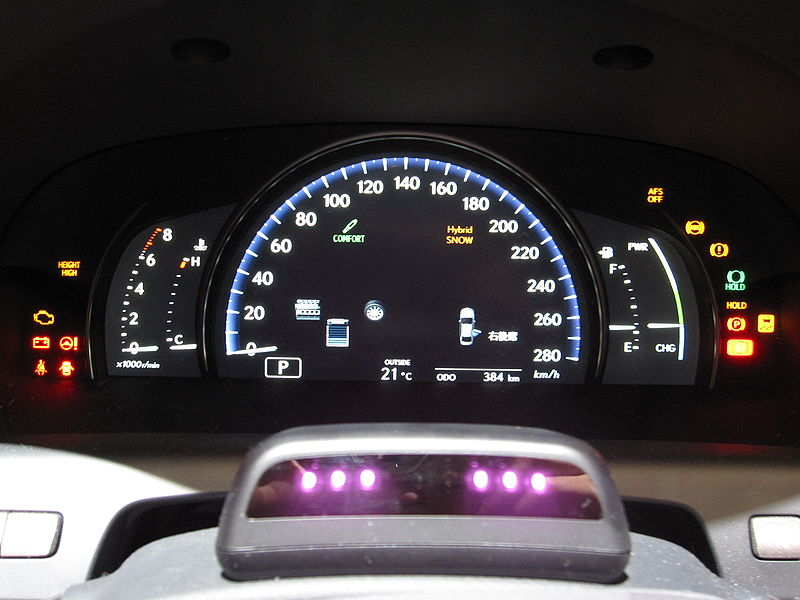
\includegraphics[width=0.7\textwidth]{images/lexus_monitoring}
\vskip10pt
\caption[Lexus Dashboard]{Lexus instrument LCD and Driver Monitoring System \cite{lexusdash}}
\label{fig:lexusdash}
\end{figure}

\subsection{Intermediate Expansion}
New technology will run concurrently with the short-term expansion goals to control a driver's cellphone notification alerts, vehicle radio, and any other additional stimuli. This will seek to reduce the distractions faced by the driver. Research into how drivers react to disturbances while driving will need to be undertaken in order to ensure the product meets its objectives.

\subsection{Long-Term Expansion}
In the not-too-distant future, the road will be filled with self-driving vehicles, similar to Google's Self-driving cars as seen in \Cref{fig:gcars}. This will make our current Uvuka Pro device redundant as drivers will not necessarily need need to be kept awake at the wheel. However, the inevitable transition period ahead will require drivers to be on alert in the event that the autonomous system is unable to navigate the vehicle. If our system detects that the occupant is not fast asleep or too drowsy to drive, warnings could be sounded and the occupant alerted to the fact that they need to take over from the automated system. Similarly, the cabin camera can be reconfigured to send signals to the car to indicate whether the occupants are awake or asleep, and adjust the driving style accordingly.

\begin{figure}[H]
\centering
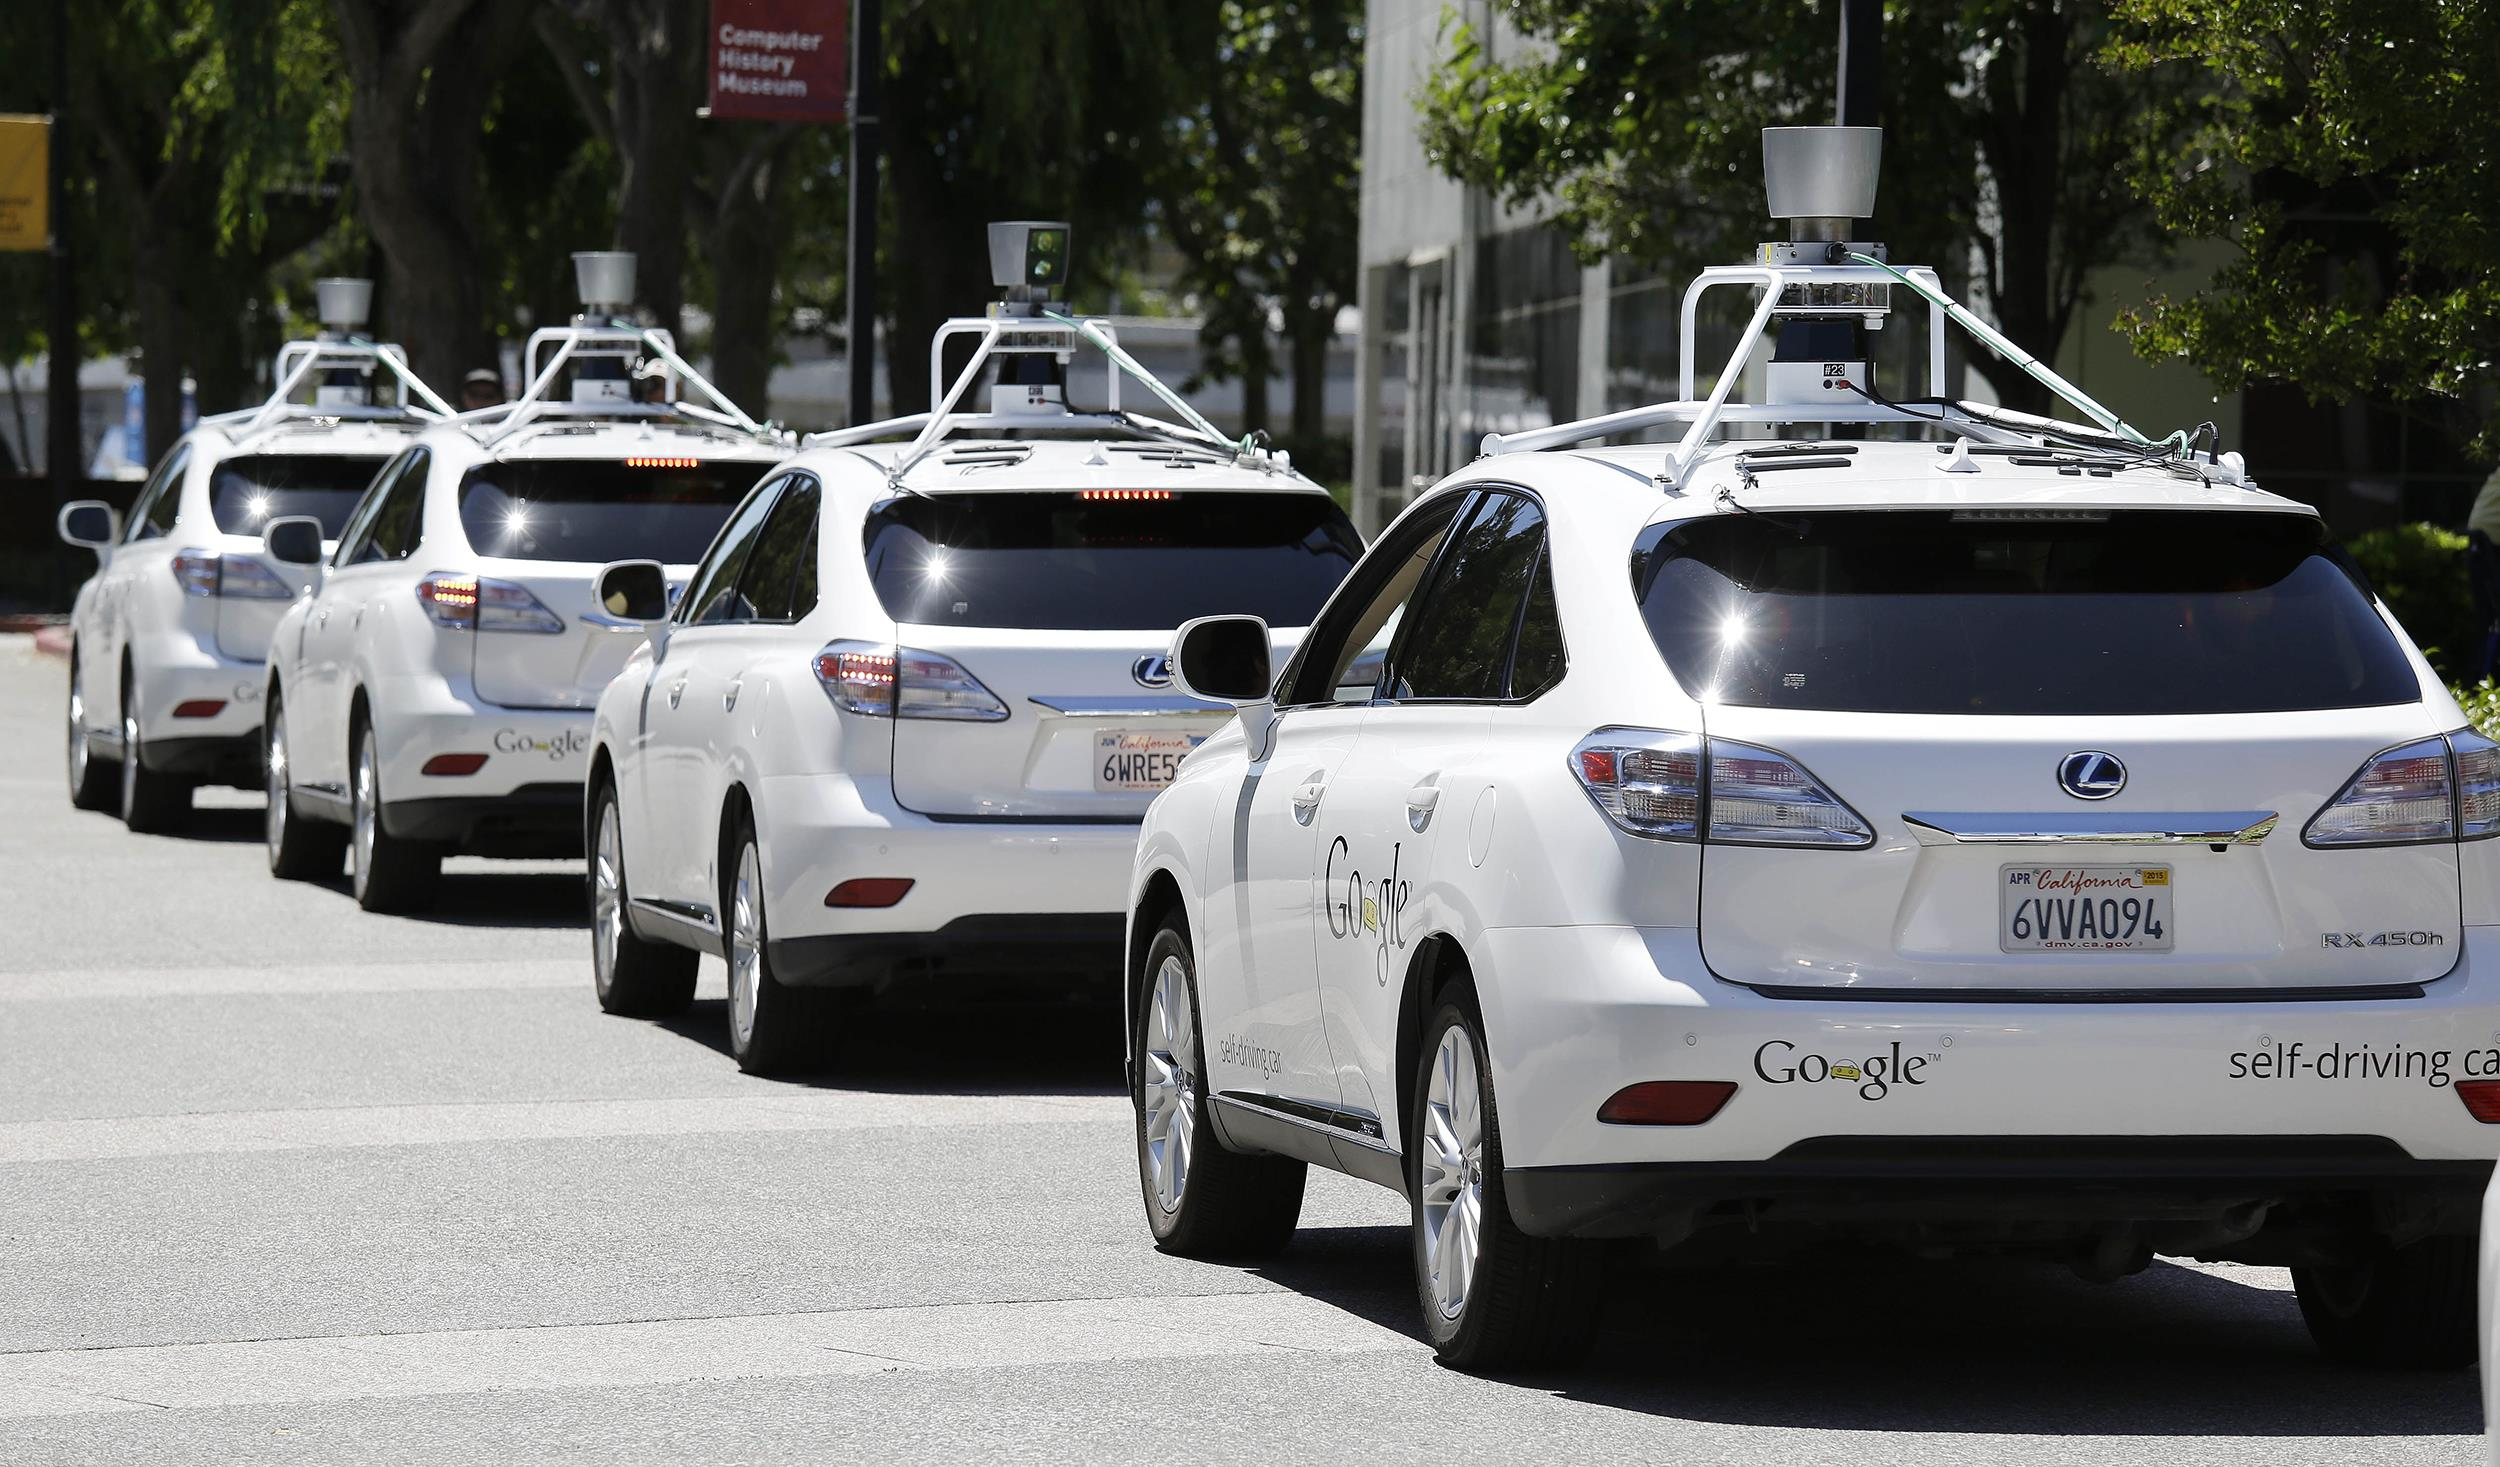
\includegraphics[width=0.7\textwidth]{images/Google_Cars}
\vskip10pt
\caption[Google's Self-driving Cars]{Google's Self-driving Cars \cite{googlecars}}
\label{fig:gcars}
\end{figure}



%\begin{appendices}
\appendix
\chapter{Insert Here}
\label{app:Insert Here}	
\newpage

\chapter{Another}
\label{app:Another}
\end{appendices}	%for use with appendices
\newpage
\renewcommand\bibname{References}
\bibliography{Aldera_bibliography}
\bibliographystyle{ieeetr}
%changing this to ^ieeetran^ and downloading the zip and compiling on Rob's PC will produce a reference list that has the URLs in it, don't worry about this for now.
\addcontentsline{toc}{chapter}{References}

\newpage	%this keeps the header/footer working on the last page. Do not type anything after this.

\end{onehalfspace}
\end{document}

%-------------------------------Figures--------------------------------%
\begin{figure}[H]
\centering
\includegraphics[width=0.4\textwidth]{images/%}
\vskip10pt
\caption[The caption that appears in the list of figures]{The caption that appears under the figure}
\label{fig:exam}
\end{figure}

\begin{figure}[H]
\centering
\begin{subfigure}[t]{0.49\textwidth}
\centering
\includegraphics[width=0.9\linewidth]{images/%}
\caption{This is figure a}
\label{fig:figureA}
\end{subfigure}
\begin{subfigure}[t]{0.49\textwidth}
\centering
\includegraphics[width=0.9\linewidth]{images/%}
\caption{This is figure b}
\label{fig:figureB}
\end{subfigure}
\caption{Caption}
\end{figure}

\begin{wrapfigure}{r}{0.5\textwidth}
\begin{center}
\includegraphics[width=0.48\textwidth]{images/ %}
\end{center}
\caption{A gull}
\end{wrapfigure}

As can be seen in \cref{fig:exam}\\
%-------------------------------Headings-------------------------------%
\chapter{Chapter Title}
\label{ch:Chapter Title}

\section{Section Title}
\label{sec:Section Title}

\subsection{Subsection Title}
\label{subsec:Subsection Title}

\subsubsection{Subsubsection Title}
\label{bb:Subsubsection Title}
%---------------------------Tables and Lists---------------------------%
\renewcommand{\contentsname}{Table of Contents} %change table of contents's name from 'contents' to 'table of contents'
\newpage %page break
\phantomsection %for some reason this gets the bookmarks to work

\tableofcontents



%\addcontentsline{toc}{chapter}{Section:} %add "table of contents" to the table of contents
\newpage %page break
\input{\filepath /list_of_figures.tex}
\input{\filepath /list_of_tables.tex}
\input{\filepath /list_of_example.tex}

\startcontents[chapters] %mini table of contents
\printcontents[chapters]{}{1}{}
\newpage
%-----------------------------Insert Pages-----------------------------%
\includepdf[pages={1}]{ %filename.pdf}
%-------------------------------Appendix-------------------------------%
\startcontents[section]
\printcontents[section]{}{1}{}
\newpage
\addcontentsline{toc}{section}{1. %}
%--------------------------------Citing--------------------------------%
\footnote{\cite{aa}}
\cite{aa,bb}
%--------------------------Custom Bibliography-------------------------%
makebst
%----------------------------Maths & Symbols---------------------------%
http://www.artofproblemsolving.com/Wiki/index.php/LaTeX:Symbols
http://www.tex.ac.uk/tex-archive/info/symbols/comprehensive/symbols-a4.pdf
$Hardcore \: maths \: here \: \therefore \ddot{\theta}^{2} = \left(\dfrac{\omega_{n}}{17a}\right) \times 9$
$$ More \: maths: \sqrt{52} + F_{1} = 6 \times 10^{5} \: Hz$$
$\mathrm{\today}$ %maths in normal font
%---------------------------Lines and Spacing--------------------------%
\noindent\makebox[\linewidth]{\rule{\textwidth}{0.4pt}}
\vspace{11pt}
\hspace{-11pt}
\hphantom{11pt}
%----------------------------Page Numbering----------------------------%
\pagenumbering{gobble} %remove page numbering
\pagenumbering{roman} %roman letters page numbering
\pagenumbering{arabic} %arabic letters page numbering
\setcounter{page}{1} %reset page numbers
%--------------------------------Tables--------------------------------%
\begin{table}[H]
\caption{Caption of table}
\addvbuffer[12pt 8pt]{
\begin{tabularx}{0.3\textwidth}{@{}rcl@{}}
\hline
\multicolumn{3}{@{}c@{}}{\textbf{Title}}\\
\hline
Info	& 3	& mm\\
Item	& 5	& x $\approx$ 34\\
\cline{2-2}
Width	& 4	& miles\\
Depth	& 7	& \pbox{20cm}{This is the first \\ cell}\\
\hline
\label{tab:capt}
\end{tabularx}
}
\end{table}

\begin{tabularx}{\textwidth}{@{}lX@{}}
 & \\
\end{tabularx}

\\
\\
\begin{tabular}{ l l }
 & \\
\end{tabular}
%--------------------------------Lists---------------------------------%
http://en.wikibooks.org/wiki/LaTeX/List_Structures

%TC:ignore
\begin{itemize} \itemsep1pt \parskip0pt \parsep0pt \vspace{-6pt}
%TC:endignore
\item[-] The first item
\item[-] The second item
\item[-] The third etc \ldots
\end{itemize}

\begin{enumerate} [label=\bfseries Exercise \arabic*:]
\item The first item
\item The second item
\item The third etc \ldots
\end{enumerate}

\begin{description}
\item[First] The first item
\item[Second] The second item
\item[Third] The third etc \ldots
\end{description}

\begin{description}
\item[First] \hfill \\
The first item
\item[Second] \hfill \\
The second item
\item[Third] \hfill \\
The third etc \ldots
\end{description}

Inline lists are \begin{enumerate*}[label=\itshape\alph*\upshape)]
\item formatted within their paragraph;
\item usually labelled with letters; and
\item usually have the final item prefixed with
`and' or `or',
\end{enumerate*} like this example.

\example{Your first example}
\label{1st_ex}
\example{Your second example}
\label{2nd_ex}
\example{Your third example. (See example \ref{1st_ex} and \ref{2nd_ex})}
%----------------------------------------------------------------------%
\fi